\setdictum{%
  Who are you? How did you get in my house?%
}{%
  Donald E. Knuth about one-based array indices in algorithms
  (according to \texttt{xkcd}\footnotemark)%
}

\longchapter{%
  Algorithms for B-Splines on Sparse Grids%
}{%
  Algorithms for B-Splines on\texorpdfstring{\\}{ }Sparse Grids%
}{%
  Algorithms for B-Splines on Sparse Grids%
}
\footnotetext{\url{https://xkcd.com/163/}}
\label{chap:40algorithms}

\initial{0.6em}{L}{ittle is known}
about the algorithmic challenges
that hierarchical bases of B-spline type (or even of general type) pose
on sparse grids.
In general, we are not able to directly apply the sparse grid algorithms
that were designed for hat functions $\bspl{l,i}{1}$.
Hence, we have to generalize these algorithms
to higher-order B-splines $\bspl{l,i}{p}$
or even to arbitrary tensor product basis functions.
The main problem is the larger support
of higher-order B-splines when compared to degree $p = 1$.
The larger support introduces new dependencies between
values of grid points that cannot be resolved with conventional algorithms.

This chapter gives an overview of six algorithms for B-splines
on sparse grids.
Two of these algorithms are already known
\multicite{Griebel92Combination,Balder94Adaptive},
while the remaining four are new.
Correctness results are given for every algorithm.
We use hierarchization as the exemplary problem for our algorithms,
but the ideas of the algorithms can be generalized to any linear operator.
Furthermore, most algorithms are not tailored to B-splines $\bspl{l,i}{p}$,
but applicable to general tensor product basis functions $\basis{l,i}$.
Whether an algorithmic approach is feasible for the sparse grid at hand
or not depends on the grid's type:
full grid, dimensionally adaptive sparse grid, or
spatially adaptive sparse grid.
The more assumptions the grid satisfies, the faster and
easier the corresponding algorithms will be.

\Cref{sec:41problem} explains hierarchization as our example problem
and defines the notation used in this chapter.
The remaining four sections treat the three different types of grids:
First, \cref{sec:42fullGrids} deals with full grids to formalize and repeat
the well-known \up.
Second, \cref{sec:43dimAdaptive} focuses on algorithms for
dimensionally adaptive sparse grids.
Third, \cref{sec:44spatAdaptiveBFS} and \cref{sec:45spatAdaptiveUP}
treat arbitrary (spatially adaptive) sparse grids,
which is the most interesting case for us.
\Cref{sec:44spatAdaptiveBFS} employs \bfs for hierarchization,
while \cref{sec:45spatAdaptiveUP} uses the \up\punctfix{.}

This original chapter is the main theoretical contribution of this thesis.
Although the unidirectional principle in \cref{sec:42fullGrids} and
the combination technique in \cref{sec:43dimAdaptive} are well-known,
the presentation with formal proofs of correctness is new.
Parts of the chapter have already been published in scientific papers,
namely \cref{sec:44spatAdaptiveBFS} \cite{Valentin18Fundamental}.
The weakly fundamental splines (\cref{sec:454wfs}) and the
Hermite hierarchization method (\cref{sec:455hermiteHierarchization})
are based on an idea by Dr.\ Stefan Zimmer (University of Stuttgart, Germany).



\section{The Hierarchization Problem}
\label{sec:41problem}

Let $\sgset \subset \clint{0, 1}^d$ be a general (sparse) grid that
may be spatially adaptive, i.e.,
of the form $\sgset = \{\gp{\*l,\*i} \mid (\*l, \*i) \in \liset\}$,
where $\liset$ is a set of level-index pairs $(\*l, \*i)$ with $\*l \in \natz^d$
and $\*i \in \hiset{\*l}$ such that
$\ngp \ceq \setsize{\sgset} = \setsize{\liset} < \infty$
(see \cref{sec:233spatiallyAdaptiveSG}).
The \term{hierarchization problem} is finding
\term{hierarchical surpluses}
$(\surplus{\*l',\*i'})_{(\*l',\*i') \in \liset} \in \real^{\ngp}$ such that
\begin{equation}
  \label{eq:hierarchizationProblem}
  \largesum{(\*l', \*i') \in \liset} \surplus{\*l',\*i'}
  \basis{\*l',\*i'}(\gp{\*l,\*i}) = \fcnval{\*l,\*i}
  \quad\text{for all}\quad
  (\*l, \*i) \in \liset,
\end{equation}
where $\basis{\*l',\*i'}$ are arbitrary tensor product basis functions and
$(\fcnval{\*l,\*i})_{(\*l,\*i) \in \liset} \in \real^{\ngp}$ is a set of
function values $\objfun(\gp{\*l,\*i})$
at the grid points $\gp{\*l,\*i}$.
This then defines the interpolant $\sgintp$ as
\begin{equation}
  \label{eq:hierarchizationInterpolant}
  \sgintp\colon \clint{\*0, \*1} \to \real,\quad
  \sgintp \ceq
  \largesum{(\*l', \*i') \in \liset} \surplus{\*l',\*i'}
  \basis{\*l',\*i'},
\end{equation}
which interpolates $\objfun$ at the grid points $\gp{\*l,\*i}$ of $\sgset$.
\Cref{fig:hierarchization} shows the process of hierarchizing given
function values and evaluating the resulting interpolant.

\begin{figure}
  \subcaptionbox{%
    The objective function $\objfun$ is sampled at the grid points
    $\gp{l,i} \in \sgset$ to obtain function values $\fcnval{l,i}$,
    which form the input vector $\vlinin$ for the linear operator
    $\linop = \intpmatinv$.%
  }[46mm]{%
    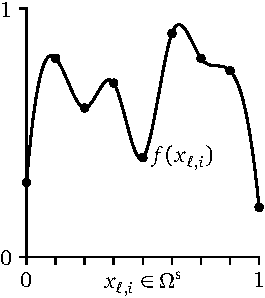
\includegraphics{hierarchization_1}%
  }%
  \hfill%
  \subcaptionbox{%
    The linear operator $\linop$ is applied to $\vlinin$ to obtain
    the output vector $\vlinout$, which contains the hierarchical surpluses
    $\surplus{l,i}$ ($(l,i) \in \liset$).%
  }[46mm]{%
    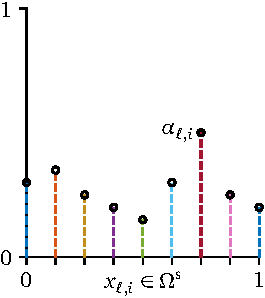
\includegraphics{hierarchization_2}%
  }%
  \hfill%
  \subcaptionbox{%
    The interpolant $\sgintp$ \emph{(black dashed line)}
    is evaluated at $x \in \clint{0, 1}$
    by adding contributions \emph{(black dotted lines)}
    of weighted basis functions $\surplus{l,i} \basis{l,i}$
    \emph{(colored),} obtaining $\sgintp(x)$ \emph{(cross).}%
  }[46mm]{%
    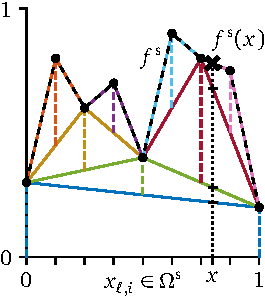
\includegraphics{hierarchization_3}%
  }%
  \caption[%
    Hierarchization of function values and evaluation of interpolant%
  ]{%
    Hierarchization of function values $\fcnval{l,i}$ \emph{(left)}
    to obtain hierarchical surpluses $\surplus{l,i}$ \emph{(center)} and
    evaluation of the resulting interpolant $\sgintp$ \emph{(right),}
    using a univariate grid and the piecewise linear basis as an example.%
  }%
  \label{fig:hierarchization}%
\end{figure}

We explicitly allow $\basis{\*l',\*i'}$ to be nodal basis functions,
in which case $\*l'$ is constant and
$\sgset$ is a full grid.
Strictly speaking, the problem is then an \term{interpolation problem}
and the $\surplus{\*l',\*i'}$ are \term{interpolation coefficients.}
However, we still apply the terms
``hierarchization'' and ``hierarchical surpluses'' in this case
to keep the terminology consistent.

\paragraph{Hierarchization as a linear operator}

The example of hierarchization can be generalized
to arbitrary linear operators
\begin{equation}
  \linop\colon \real^{\ngp} \to \real^{\ngp},\quad
  \vlinin \mapsto \vlinout = \linop[\vlinin],
\end{equation}
where $\linop$ depends on the grid $\sgset$ at hand.
Input $\vlinin$ and output $\vlinout$ are scalar-valued data%
\begin{equation}
  \vlinin = (\linin{\*l,\*i})_{(\*l,\*i) \in \liset} \in \real^{\ngp},\quad
  \vlinout = (\linout{\*l,\*i})_{(\*l,\*i) \in \liset} \in \real^{\ngp},
\end{equation}
which give one scalar per grid point $\gp{\*l,\*i} \in \sgset$.
For the case of hierarchization,
$\linop$ is the inverse of the \term{interpolation matrix}
$\intpmat \in \real^{\ngp \times \ngp}$:
\begin{subequations}
  \label{eq:hierarchizationSLE}
  \begin{equation}
    \linop = \intpmatinv,\quad
    \intpmat = (\basis{\*l',\*i'}(\gp{\*l,\*i}))_%
    {(\*l,\*i),(\*l',\*i') \in \liset},\quad
    \vlinin = (\fcnval{\*l,\*i})_{(\*l,\*i) \in \liset},\quad
    \vlinout = (\surplus{\*l',\*i'})_{(\*l',\*i') \in \liset}.
    \hspace*{-1mm}
  \end{equation}
  This means that we can determine the $\surplus{\*l',\*i'}$ by solving
  the $\ngp \times \ngp$ system of linear equations
  \begin{equation}
    \vlinout = \linop[\vlinin]
    \quad\iff\quad
    \intpmat \cdot (\surplus{\*l',\*i'})_{(\*l',\*i') \in \liset}
    = (\fcnval{\*l,\*i})_{(\*l,\*i) \in \liset}.
  \end{equation}
\end{subequations}

\paragraph{Complexity of B-spline hierarchization}

As noted in \cite{Valentin18Fundamental},
hierarchization on sparse grids with hierarchical B-splines
$\bspl{\*l,\*i}{\*p}$ of degree $\*p$
as basis functions $\basis{\*l,\*i}$ is a tedious task.
The corresponding linear system \eqref{eq:hierarchizationSLE} is in general
non-symmetric
(i.e., $\bspl{\*l',\*i'}{\*p}(\gp{\*l,\*i}) \not=
\bspl{\*l,\*i}{\*p}(\gp{\*l',\*i'})$) and densely populated.
This is because the matrix entry in the $(\*l,\*i)$-th row and
$(\*l',\*i')$-th column vanishes if and only if
\begin{equation}
  \gp{\*l,\*i} \notin \interiorsupp \bspl{\*l',\*i'}{\*p}
  \iff
  \exlarge{t = 1, \dotsc, d}{
    \gp{l_t,i_t} \notin
    \opintscaled{
      \gp{l'_t,i'_t} - \tfrac{p_t+1}{2} \ms{l'_t},\,
      \gp{l'_t,i'_t} + \tfrac{p_t+1}{2} \ms{l'_t}
    }
  },
\end{equation}
where $\interiorsupp$ is the interior of the support
\cite{Valentin18Fundamental}.
For coarse levels $\*l'$, the mesh size $\ms{l'_t}$ is large in
every dimension $t$, which implies that $\interiorsupp \bspl{\*l',\*i'}{\*p}$
contains most of the grid points.
In contrast to the hat function case ($\*p = \*1$),
the value of $\surplus{\*l',\*i'}$ depends not only on
$\fcnval{\*l,\*i}$ and the data of the $3^d - 1$ neighboring grid points
on the boundary of $\supp \bspl{\*l',\*i'}{\*1}$,
but potentially on the data of the whole grid.
This is shown in \cref{fig:matrixDensityPattern}:
There are at most $3^d = 9$ non-zero entries in each row of $\intpmatinv$
for $\*p = \*1$ and $d = 2$.
As soon as the B-spline degree is increased,
both $\intpmat$ and $\intpmatinv$ become significantly denser.

\begin{SCfigure}
  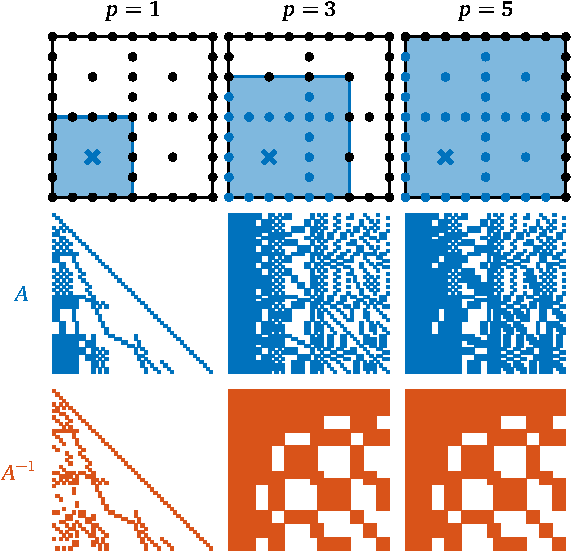
\includegraphics{matrixDensityPattern_1}%
  \caption[%
    Density pattern of hierarchization matrices and of their inverses%
  ]{%
    Density pattern
    of the hierarchization matrix $\intpmat$
    \emph{(middle row, \textcolor{C0}{blue})} and
    of its inverse $\intpmatinv$
    \emph{(bottom row, \textcolor{C1}{red})}
    for the regular sparse grid $\coarseregsgset{n}{d}{1}$
    with $n = 4$ and $d = 2$ \emph{(top row)}
    and uniform hierarchical B-splines $\bspl{\*l,\*i}{\*p}$
    for degrees $\*p \in \{\*1, \*3, \*5\}$.
    The \textcolor{C0}{blue areas} in the top row
    show the extent of the support of one specific basis function
    $\bspl{\*l',\*i'}{\*p}$ with $\*l' = (2, 2)$ and $\*i' = (1, 1)$
    (\emph{cross:} corresponding grid point $\gp{\*l',\*i'}$).
    The \textcolor{C0}{blue points} are the grid points at which
    $\bspl{\*l',\*i'}{\*p}$ is non-zero.%
  }%
  \label{fig:matrixDensityPattern}%
\end{SCfigure}

This prohibits the use of the \up\punctfix{,}
which we will discuss in the next section,
on sparse grids with hierarchical B-splines.
Consequently, we have to solve the linear system
\eqref{eq:hierarchizationSLE}, which is significantly more time-consuming,
as it takes between $\landauOmega{\ngp^2 d}$ and $\landauO{\ngp^2 (N+d)}$ time
via Gaussian elimination.%
\footnote{%
  $\landauOmega{\ngp^2 d}$ for assembling $\intpmat$ and
  $\landauO{\ngp^3}$ for solving the system.
}
In addition, if we use an explicit solver for the linear system,
we additionally have to store an $\ngp \times \ngp$ matrix in memory.
However, a grid of size $\ngp = \num{116000}$ already exceeds the memory
of a \SI{128}{\gibi\byte} supercomputer node,
if we explicitly store the full matrix in double precision.
In comparison, for the hat function basis,
the \up only requires $\landauO{\ngp d}$ time and $\landauO{\ngp}$ memory.

\paragraph{Notation}

We do not need the hierarchical level-index information $(\*l, \*i)$ in
$\sgset$, $\liset$, $\vlinin$, and $\vlinout$
for most of the considerations in this chapter.
In these cases, we assume that in each dimension $t$, the level-index pairs
$(l_t, i_t)$ ($l_t \in \natz$, $i_t \in \hiset{l_t}$)
are continuously enumerated by a single index $k_t = k_t(l_t, i_t) \in \natz$.
We identify $(\*l, \*i)$ with a single index $\*k$,
whose $t$-th component is given by $k_t(l_t, i_t)$.
Hence,
we regard $\liset$ as a subset $\liset \ceq \{\*k \mid \*x_\*k \in \sgset\}$
of $\natz^d$.
We will switch between the notations whenever appropriate.
All statements that are formulated in the $\*k$ notation are
valid for both the nodal and the hierarchical basis.

\usenotation{kT00}
In the following, $k_t$ denotes the $t$-th component of a $d$-vector $\*k$
as usual.
\usenotation{kT10}
With $\*k_{-t}$, we denote the $(d-1)$-vector that is obtained from $\*k$
by omitting the $t$-th component,
i.e., $\*k_{-t} \ceq (k_1, \dotsc, k_{t-1}, k_{t+1}, \dotsc, k_d)$.
\usenotation{kT20}
For a $j$-tuple $T = (t_1, \dotsc, t_j) \in \{1, \dotsc, d\}^j$,
we define $\*k_T$ to be the $j$-vector $(k_{t_1}, \dotsc, k_{t_j})$
that only contains the entries of the dimensions listed in $T$.
\usenotation{kT30}
Accordingly, $\*k_{-T}$ is defined as the $(d-j)$-vector
that contains the entries of the remaining dimensions
(sorted by the dimension $t$).
We define $\*k_{\range{a}{b}} \ceq (k_a, k_{a+1}, \dotsc, k_b)$
as an indexing shortcut ($a \le b$).

\section{Hierarchization on Full Grids (Unidirectional Principle)}
\label{sec:42fullGrids}

If $\sgset$ is a full grid $\fgset{\*l}$
(see \cref{sec:21nodalSpaces}),
the well-known \up
can be used to apply $\linop$ to input data $\vlinin$.
As shown in \cref{fig:unidirectionalPrinciple} for a sparse grid,
the idea of the \up
is to apply the corresponding one-dimensional operators on the
one-dimensional subgrids (the \term{poles}) of $\sgset$,
which is repeated for all dimensions.
In this section, we first formulate the \up for
general linear operators $\linop$ and then prove its correctness for
the case $\linop = \intpmatinv$ of hierarchization.
The correctness for arbitrary tensor product operators
will follow from \cref{sec:45spatAdaptiveUP}.

\begin{figure}
  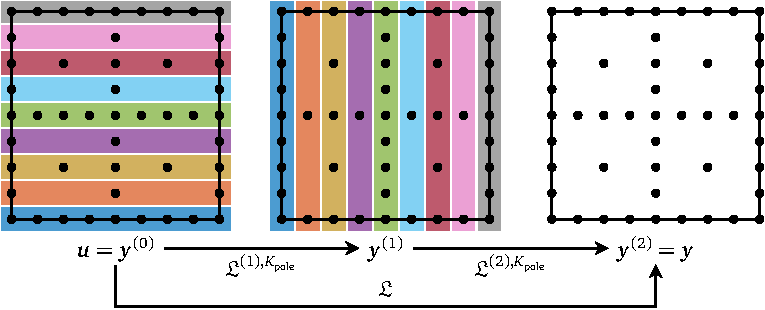
\includegraphics{unidirectionalPrinciple_1}%
  \caption[%
    Unidirectional principle%
  ]{%
    Application of a linear operator $\linop$
    on two-dimensional sparse grid data with the unidirectional principle.
    \emph{Left:}
    The univariate operator $\upopuv{1}{\lisetpole}$ is applied on
    the input data $\vlinin$
    along poles $\lisetpole$ of the first dimension $x_1$.
    \vspace{-0.2em}%
    \emph{Center:}
    The univariate operator $\upopuv{2}{\lisetpole}$ is applied on the
    resulting intermediate data $\vlinout[(1)]$
    along poles $\lisetpole$ of the second dimension $x_2$.
    \emph{Right:}
    Final values $\vlinout = \linop[\vlinin]$ after the application
    on both dimensions.
    All grid points of the same color are part of the same pole $\lisetpole$
    (equivalence classes of $\samepole{t}$ in
    \cref{alg:unidirectionalPrinciple}).%
  }%
  \label{fig:unidirectionalPrinciple}%
\end{figure}

\paragraph{Unidirectional principle and its correctness}

We state the \up in \cref{alg:unidirectionalPrinciple}.
The algorithm is given a permutation $(t_1, \dotsc, t_d)$ of $(1, \dotsc, d)$
that specifies the order of dimensions in which the \up should be applied.
We denote with $\upopuv{t_j}{\lisetpole}$ the one-dimensional version of $\linop$
applied in dimension $t_j$ ($j = 1, \dotsc, d$) on the pole $\lisetpole$.
Formally, a pole is an equivalence class of the
\term{pole equivalence relation} $\samepole{t_j}$ on $\liset$:
\begin{equation}
  \label{eq:poleEquivalenceRelation}
  \*k' \samepole{t_j} \*k'' \iff \*k'_{-t_j} = \*k''_{-t_j},\quad
  \*k', \*k'' \in \liset.
\end{equation}
We prove the correctness of the \up with the following invariant:

\begin{algorithm}
  \begin{algorithmic}[1]
    \Function{$\vlinout = \texttt{unidirectionalPrinciple}$}{%
      $\vlinin$, $\liset$, $(t_1, \dotsc, t_d)$%
    }
      \State{$\vlinout[(0)] \gets \vlinin$}
      \For{$j = 1, \dotsc, d$}
        \For{$\lisetpole \in \eqclasses{\liset}{\samepole{t_j}}$}
          \State{%
            $(\linout[(j)]{\*k})_{\*k \in \lisetpole} \gets
            \upopuv{t_j}{\lisetpole}
            \bracket*{(\linout[(j-1)]{\*k})_{\*k \in \lisetpole}}$%
          }
          \Comment{apply univariate operator on pole}%
          \label{line:algUnidirectionalPrinciple1}
        \EndFor{}
      \EndFor{}
      \State{$\vlinout \gets \vlinout[(d)]$}
    \EndFunction{}
  \end{algorithmic}
  \caption[%
    Unidirectional principle%
  ]{%
    Application of a tensor product operator $\linop$ with
    the unidirectional principle.
    Inputs are
    the vector $\vlinin = (\linin{\*k})_{\*k \in \liset}$ of input data,
    the set $\liset$ of grid indices, and
    the permutation $(t_1, \dotsc, t_d)$ specifying the order in which
    the one-dimensional operators $\upopuv{t_j}{\lisetpole}$ should be applied.
    The output is the vector $\vlinout = (\linout{\*k})_{\*k \in \liset}$
    of output data.%
  }%
  \label{alg:unidirectionalPrinciple}%
\end{algorithm}

\begin{proposition}[invariant of unidirectional principle for hierarchization]
  \label{prop:invariantUnidirectionalPrinciple}
  Let $\linop$ be the hierarchization operator on a full grid,
  i.e.,
  $\linop = \intpmatinv$,
  $\vlinin = (\fcnval{\*k})_{\*k \in \liset}$,
  $\vlinout = (\surplus{\*k})_{\*k \in \liset}$,
  $\upopuv{t_j}{\lisetpole}$ is the univariate interpolation operator
  $\intpmatuvinv{t_j}$, and
  $\liset = \{\*0, \dotsc, \*2^\*l\}$
  corresponds to a full grid $\fgset{\*l}$ of level $\*l$.
  After iteration $j$ of \cref{alg:unidirectionalPrinciple}
  ($j = 1, \dotsc, d$), it holds for $T \ceq (t_1, \dotsc, t_j)$
  \begin{equation}
    \sum_{\*k_T=\*0}^{\*2^{\*l_T}}
    \linout[(j)]{(\*k_T,\*k'_{-T})} \basis{\*k_T}(\gp{\*k'_T})
    = \fcnval{\*k'},\quad
    \*k' = \*0, \dotsc, \*2^\*l,
  \end{equation}
  where $(\*k_T,\*k'_{-T})$ is shorthand for $\*k''$
  with $k''_t \ceq k_t$ if $t \in T$ and $k''_t \ceq k'_t$ if $t \notin T$.
\end{proposition}

\begin{proof}
  We prove the assertion by induction over $j = 1, \dotsc, d$.
  We set $T' \ceq (t_1, \dotsc, t_{j-1})$,
  $T \ceq (t_1, \dotsc, t_{j-1}, t_j)$,
  and we exploit the tensor product structure of the basis
  to write the \lhs of the assertion for $j$
  and arbitrary $\*k' = \*0, \dotsc, \*2^\*l$ as
  \begin{equation}
    \label{eq:proofPropInvariantUnidirectionalPrinciple1}
    \sum_{\*k_T=\*0}^{\*2^{\*l_T}}
    \linout[(j)]{(\*k_T,\*k'_{-T})} \basis{\*k_T}(\gp{\*k'_T})
    = \sum_{\*k_{T'}=\*0}^{\*2^{\*l_{T'}}}
    \basis{\*k_{T'}}(\gp{\*k'_{T'}})
    \sum_{k_{t_j}=0}^{2^{l_{t_j}}}
    \linout[(j)]{(\*k_T,\*k'_{-T})} \basis{k_{t_j}}(\gp{k'_{t_j}}).
  \end{equation}
  If we choose the equivalence class
  $\lisetpole \ceq \eqclass{(\*k_T,\*k'_{-T})}{\samepole{t_j}}$
  ($\*k_T$ arbitrary),
  then the inner sum over $k_{t_j}$ equals
  \begin{equation}
    \label{eq:proofPropInvariantUnidirectionalPrinciple2}
    \sum_{\*k'' \in \lisetpole}
    \linout[(j)]{\*k''} \basis{k''_{t_j}}(\gp{k'_{t_j}})
    = \paren*{
      (\upopuv{t_j}{\lisetpole})^{-1}
      \bracket*{(\linout[(j)]{\*k''})_{\*k'' \in \lisetpole}}
    }_{k'_{t_j}}
    = \linout[(j-1)]{(\*k_{T'},\*k'_{-T'})}
  \end{equation}
  by \cref{line:algUnidirectionalPrinciple1} of
  \cref{alg:unidirectionalPrinciple}.
  We can conclude that the \lhs
  \cref{eq:proofPropInvariantUnidirectionalPrinciple1} equals
  \begin{equation}
    \sum_{\*k_{T'}=\*0}^{\*2^{\*l_{T'}}}
    \linout[(j-1)]{(\*k_{T'},\*k'_{-T'})}
    \basis{\*k_{T'}}(\gp{\*k'_{T'}}),
  \end{equation}
  which, by the induction hypothesis, equals $\fcnval{\*k'}$ as desired
  (if $j > 1$).
  The same reasoning for
  \eqref{eq:proofPropInvariantUnidirectionalPrinciple2} can be used
  to establish the base case for $j = 1$.
\end{proof}

\begin{shortcorollary}[%
  correctness of unidirectional principle for hierarchization%
]
  \label{cor:algUnidirectionalPrincipleCorrectness}
  \Cref{alg:unidirectionalPrinciple}
  is correct for hierarchization on full grids.
\end{shortcorollary}

\begin{proof}
  We apply \cref{prop:invariantUnidirectionalPrinciple} for $j = d$ to obtain
  $\sum_{\*k=\*0}^{\*2^\*l}
  \linout[(j)]{\*k} \basis{\*k}(\gp{\*k'})
  = \fcnval{\*k'}$
  for all $\*k' = \*0, \dotsc, \*2^\*l$, i.e.,
  the $\linout[(j)]{\*k}$ are the correct interpolation coefficients
  according to \eqref{eq:hierarchizationProblem}.
\end{proof}

\paragraph{Complexity}

We compare the complexity of the \up for hierarchization with
the direct solution of the system \eqref{eq:hierarchizationSLE} of
linear equations.
If we assume that $d$ is constant and that
$\linop$ and $\upopuv{t_j}{\lisetpole}$ apply Gaussian elimination to
solve the multivariate and univariate systems, respectively,
then directly solving \eqref{eq:hierarchizationSLE} takes
$\landauO{\ngp^2 (\ngp + d)}$ time and
$\landauO{\ngp^2}$ memory.
In contrast, the \up only requires
$\landauO{\ngp \sum_t \ngp_t^2}$ time%
\footnote{%
  There are $\ngp/\ngp_t$ poles in the
  $t$-th iteration of \cref{alg:unidirectionalPrinciple}.
  Each pole requires the solution of an $\ngp_t \times \ngp_t$ linear system,
  which takes $\landauO{\ngp_t^3}$ time.%
}
and $\landauO{\max\{N_1^2, \dotsc, N_d^2, N\}}$ memory,
where $\ngp_t$ is the grid size
$\setsize{\{k_t \mid \*k \in \liset\}}$ in dimension $t = 1, \dotsc, d$.
The dependency from the univariate grid sizes $\ngp_t$ instead of $\ngp$
makes the \up significantly less computationally expensive.
As already mentioned,
the \up is even more efficient in the piecewise linear case,
where the univariate interpolation operators can be applied
in-place.
Hence, it only needs $\landauO{Nd}$ time and
$\landauO{N}$ memory in this case.

\section{Hierarchization on Dimensionally Adaptive Sparse Grids}
\label{sec:43dimAdaptive}

\minitoc{77mm}{7}

\noindent
Dimensionally adaptive sparse grids,
which are sums of different hierarchical subspaces
as described in \cref{sec:232dimensionallyAdaptiveSG},
have the advantage over general spatially adaptive sparse grids
that algorithms can be formulated and applied more easily.
In this section, we describe two methods:
first, the well-known combination technique, which was
already mentioned in \cref{sec:232dimensionallyAdaptiveSG},
and second, a new algorithm based on residual interpolation.



\subsection{The Combination Technique and Its Combinatorial Proof}
\label{sec:431combiTechniqueProof}

The combination technique was one of the first methods that
were developed by Griebel et al. in \cite{Griebel92Combination}
(for two and three dimensions)
after the term ``sparse grids'' was coined in 1991 \cite{Zenger91Sparse}.
However, the combination technique predates the development of sparse grids
by decades, as it was already mentioned by Smolyak in 1963
\multicite{Smolyak63Quadrature,Hegland07Combination}.
Delvos developed and proved the standard combination formula in the
framework of Boolean interpolation operators in 1982
\multicite{Delvos82Dvariate,Delvos89Boolean}.

\paragraph{Formal description and outline of a combinatorial proof}

In the following, we give a formal description of the
sparse grid combination technique, and we outline a new combinatorial proof
of its correctness.
While we discuss a high-level explanation of the proofs in this section,
the proofs themselves can be found in \cref{sec:a131proofCombiTechnique},
since most of them are rather technical.
For simplicity,
we formulate the combination technique and its proof for regular
sparse grids (see \cref{sec:231regularSG}).
However, the main ideas of the chain of proofs are also applicable
to dimensionally adaptive sparse grids
(see \cref{sec:232dimensionallyAdaptiveSG}).

\begin{theorem}[sparse grid combination technique]
  \label{thm:combiTechnique}
  Let $\liset \ceq \{(\*l, \*i) \mid
  \normone{\*l} \le n,\; \*i \in \hiset{\*l}\}$
  correspond to the regular sparse grid
  $\regsgset{n}{d}$ and let $(\fcnval{\*l,\*i})_{(\*l,\*i) \in \liset}$
  be given function values on $\regsgset{n}{d}$.
  If we define
  \begin{itemize}
    \item
    the combined sparse grid interpolant $\regsgintp[\ct]{n}{d}$ via
    \eqref{eq:combiTechnique}, i.e.,
    \begin{equation}
      \regsgintp[\ct]{n}{d}
      = \sum_{q=0}^{d-1} (-1)^q \binom{d-1}{q} \sum_{\normone{\*l'} = n-q}
      \fgintp{\*l'},
    \end{equation}
    where $\fgintp{\*l'} \in \ns{\*l'}$ is the full grid interpolant
    of $\objfun$ with level $\*l'$, and
    
    \item
    the hierarchical sparse grid interpolant $\regsgintp{n}{d}$
    via \eqref{eq:hierarchizationProblem} and
    \eqref{eq:hierarchizationInterpolant}
  \end{itemize}
  and if we assume that the hierarchical splitting equation
  \eqref{eq:hierSplittingMV} holds,
  then the combined and the hierarchical sparse grid interpolants coincide:
  \begin{equation}
    \regsgintp[\ct]{n}{d}
    = \regsgintp{n}{d}.
  \end{equation}
\end{theorem}

\begin{proof}[Proof (sketch)]
  Let $\gp{\*l,\*i} \in \regsgset{n}{d}$ be an arbitrary
  point of the regular sparse grid.
  First, we split the inner sum of $\regsgintp[\ct]{n}{d}(\gp{\*l,\*i})$
  into levels $\*l'$ whose full grid sets $\fgset{\*l'}$
  contain $\gp{\*l,\*i}$ and levels whose full grid sets
  do not contain $\gp{\*l,\*i}$:
  \begin{equation}
    \regsgintp[\ct]{n}{d}(\gp{\*l,\*i})
    = \sum_{q=0}^{d-1} (-1)^q \binom{d-1}{q} \cdot \paren*{
      \sum_{\substack{\normone{\*l'} = n - q\\\fgset{\*l'} \ni \gp{\*l,\*i}}}
      \fgintp{\*l'}(\gp{\*l,\*i}) +
      \sum_{\substack{\normone{\*l'} = n - q\\\fgset{\*l'} \notni \gp{\*l,\*i}}}
      \fgintp{\*l'}(\gp{\*l,\*i})
    }.
  \end{equation}
  The summands $\fgintp{\*l'}(\gp{\*l,\*i})$ of the first inner sum
  each equal $\fcnval{\*l,\*i}$ due to the full grid interpolation
  property \eqref{eq:interpFullGridMV}.
  Therefore, the first inner sum is equal to the product of
  $\fcnval{\*l,\*i}$ with the number of summands:
  \begin{equation}
    \label{eq:combiTechniqueSplitSum}
    \begin{split}
      \regsgintp[\ct]{n}{d}(\gp{\*l,\*i})
      &= \fcnval{\*l,\*i} \cdot \sum_{q=0}^{d-1} (-1)^q \binom{d-1}{q} \cdot
      \setsize{
        \{\*l' \mid \normone{\*l'} = n - q,\; \fgset{\*l'} \ni \gp{\*l,\*i}\}
      }\\
      &\qquad{} {} + \sum_{q=0}^{d-1} (-1)^q \binom{d-1}{q} \cdot
      \sum_{\substack{\normone{\*l'} = n - q\\\fgset{\*l'} \notni \gp{\*l,\*i}}}
      \fgintp{\*l'}(\gp{\*l,\*i}).
    \end{split}
  \end{equation}
  After this sketch of proof,
  we will prove that the first of the two summands in
  \cref{eq:combiTechniqueSplitSum}
  equals one (see \cref{prop:combiTechniqueOne})
  and that the second of the two summands
  equals zero (see \cref{prop:combiTechniqueZero}).
  Consequently, we infer
  \begin{equation}
    \regsgintp[\ct]{n}{d}(\gp{\*l,\*i})
    = \fcnval{\*l,\*i},
  \end{equation}
  i.e., $\regsgintp[\ct]{n}{d}$ interpolates $\objfun$ at $\regsgset{n}{d}$.
  Note that $\regsgintp[\ct]{n}{d}$ is contained in $\regsgspace{n}{d}$,
  if the hierarchical splitting equation \eqref{eq:hierSplittingMV} holds,
  as
  \begin{equation}
    \fgintp{\*l'} \in
    \ns{\*l'}
    = \bigoplus_{\*l''=\*0}^{\*l'} \hs{\*l''}
    \subset \regsgspace{n}{d},\quad
    \normone{\*l'} \le n,
  \end{equation}
  due to $\normone{\*l''} \le \normone{\*l'} \le n$
  for $\*l'' \le \*l'$, i.e.,
  $\hs{\*l''} \subset \regsgspace{n}{d}$ for
  $\*l'' = \*0, \dotsc, \*l'$.%
  \footnote{%
    This argumentation can be straightforwardly adapted
    for general dimensionally adaptive sparse grids
    with downward closed level sets as mentioned in
    \cref{sec:232dimensionallyAdaptiveSG}.%
  }
  As both $\regsgintp[\ct]{n}{d}$ and $\regsgintp{n}{d}$
  are contained in $\regsgspace{n}{d}$ and
  interpolate $\objfun$ on $\regsgset{n}{d}$, they coincide
  due to the uniqueness of sparse grid interpolation
  (linear independence of the hierarchical basis).
\end{proof}

\paragraph{Inclusion-exclusion principle}

It remains to prove that the first sum in \eqref{eq:combiTechniqueSplitSum}
is indeed one and that the second sum vanishes.
The first statement is a direct consequence of the
\term{inclusion-exclusion principle} \cite{Hegland07Combination}.
In its simplest form, the idea of the principle is that the cardinality
of the union of two finite subsets $A$ and $B$ of some set is given by
\begin{equation}
  \setsize{A \cup B}
  = \setsize{A} + \setsize{B} - \setsize{A \cap B},
\end{equation}
i.e., we first count (include)
the elements in $A$ and then in $B$,
but as we have counted the elements of $A \cap B$ twice,
we have to subtract (exclude) its cardinality again.

The setting is similar for the combination technique.
If we add all grids in \cref{fig:combinationTechnique}
on the green diagonal, then every point whose index is not odd
will be counted multiple times.
By subtracting the number of occurrences of the points on the
red diagonal,
the result of the ``weighted counting'' is exactly one for every point.
The following proposition, whose proof is of purely combinatorial nature,
generalizes this argument to higher dimensions:

\begin{restatable}[inclusion-exclusion principle]{%
  proposition%
}{%
  propCombiTechniqueOne%
}
  \label{prop:combiTechniqueOne}
  For every $\gp{\*l,\*i} \in \regsgset{n}{d}$, we have
  \begin{equation}
    \label{eq:combiTechniqueOne}
    \sum_{q=0}^{d-1} (-1)^q \binom{d-1}{q} \cdot
    \setsize{
      \{\*l' \mid \normone{\*l'} = n - q,\; \fgset{\*l'} \ni \gp{\*l,\*i}\}
    }
    = 1.
  \end{equation}
\end{restatable}

\begin{proof}
  See \cref{sec:a131proofCombiTechnique}.
\end{proof}

\paragraph{Canceling out function values}

The second statement about the vanishing second sum in
\eqref{eq:combiTechniqueSplitSum} is much harder to prove.
It says that at every grid point $\gp{\*l,\*i}$,
the contributions $\fgintp{\*l'}$ of levels $\*l'$
that do not contain that point cancel out,
which may seem quite surprising.
The key observation is as follows:
The values of $\fgintp{\*l'}, \fgintp{\*l''}$ for two levels
$\*l', \*l''$ are the same at $\gp{\*l,\*i}$,
if all non-equal entries $l'_t, l''_t$ of the levels are
each greater or equal to $l_t$.

For a higher-level explanation,
note that the statement $l'_t \ge l_t$ is equivalent to
$\fgset{l'_t} \ni \gp{l_t,i_t}$.
Both $\fgintp{\*l'}, \fgintp{\*l''}$ interpolate at
$\gp{\*l,\*i}$ when projected onto the $t$-th dimension,
so their contribution to $\fgintp{\*l'}(\gp{\*l,\*i})$ and
$\fgintp{\*l''}(\gp{\*l,\*i})$ must be the same.
Although there may be dimensions $t$ for which
$\fgset{l'_t} \notni \gp{l_t,i_t}$,
these dimensions do not matter if $l'_t = l''_t$,
as the univariate restrictions of $\fgintp{\*l'}, \fgintp{\*l''}$
interpolate the same data, and they are evaluated at the same point
$\gp{l_t,i_t}$.

One can formalize these considerations by defining an
equivalence relation on the set of levels such that the values of
$\fgintp{\*l'}$ at $\gp{\*l,\*i}$ are constant
on the equivalence classes.

\begin{definition}[%
  equivalence relation for the proof of the combination technique%
]
  \label{def:combiTechniqueEquivalenceRelation}
  Let $\gp{\*l,\*i} \in \regsgset{n}{d}$ be fixed and
  \begin{equation}
    \label{eq:combiTechniqueSpecialLevelSet}
    L
    \ceq \{\*l' \mid \ex{q=0,\dotsc,d-1}{
      \normone{\*l'} = n - q,\; \fgset{\*l'} \notni \gp{\*l,\*i}
    }\}
  \end{equation}
  be the set of levels that do not contain $\gp{\*l,\*i}$.
  We define a relation $\eq$ on $L$ as follows:
  For $\*l', \*l'' \in L$, we set $\*l' \eq \*l''$ if and only if
  \begin{equation}
    \falarge{t \notin T_{\*l',\*l''}}{\min\{l'_t, l''_t\} \ge l_t},\quad
    T_{\*l',\*l''}
    \ceq \{t \mid l'_t = l''_t < l_t\}.
  \end{equation}
\end{definition}

\begin{restatable}[identical values in equivalence classes]{%
  shortlemma%
}{%
  lemmaCombiTechniqueIdenticalValues%
}
  \label{lemma:combiTechniqueIdenticalValues}
  Let $\*l', \*l'' \in L$ with $\*l' \eq \*l''$.
  Then, $\fgintp{\*l'}(\gp{\*l,\*i})
  = \fgintp{\*l''}(\gp{\*l,\*i})$.
\end{restatable}

\begin{proof}
  See \cref{sec:a131proofCombiTechnique}.
\end{proof}

By exploiting the tensor product structure of the basis functions,
the proof shows an even stronger version, which is shown
in \cref{fig:combiTechniqueProof}:
The components $\fgintp{\*l'}$ and $\fgintp{\*l''}$ are equal
on the $m$-dimensional affine subspace through $\gp{\*l,\*i}$
parallel to the $m$ coordinates in $T_{\*l',\*l''}$
(where $m \ceq \setsize{T_{\*l',\*l''}}$).
The lemma allows us to group summands in the second sum of
\eqref{eq:combiTechniqueSplitSum} by function values.
Hence, it remains to count the number of levels in
each equivalence class of $\eq$.
Therefore, we need a characterization of the equivalence classes:

\begin{SCfigure}
  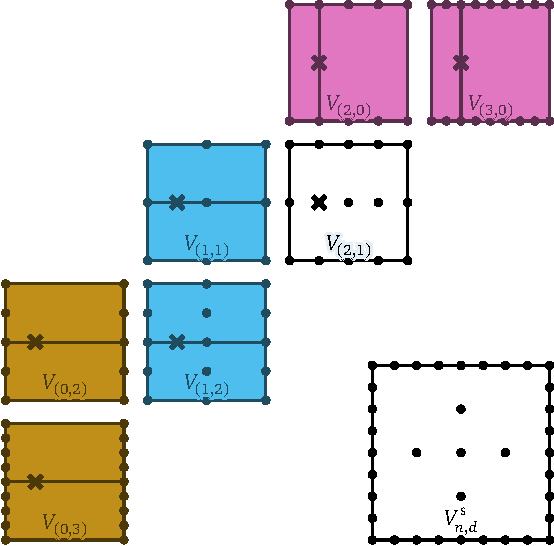
\includegraphics{combiTechniqueProof_1}%
  \caption[%
    Canceling out function values in the proof of the combination technique%
  ]{%
    Nodal subspaces $\ns{\*l}$ contributing to the combination
    technique solution for the two-dimensional regular sparse grid
    $\regsgspace{n}{d}$ of level $n = 3$ \emph{(bottom right).}
    After picking a point $\gp{\*l,\*i} \in \regsgset{n}{d}$
    (\emph{cross,} here $\*l = (2, 1)$, $\*i = (1, 1)$),
    the set $L$ of levels whose grids do not contain $\gp{\*l,\*i}$
    \emph{(colored subspaces)}
    decompose into three disjoint equivalence classes
    \emph{(colors)} given by the relation $\eq$.
    In every equivalence class $L_0 \in \eqclasses{L}{\eq}$,
    the interpolants $\fgintp{\*l'}$ ($\*l' \in L_0$)
    equal on an affine subspace
    \emph{(dark lines),} which contains $\gp{\*l,\*i}$.
    Due to the combination coefficients,
    the contribution to the combined solution
    vanishes per equivalence class.%
  }%
  \label{fig:combiTechniqueProof}%
\end{SCfigure}

\begin{restatable}[characterization of equivalence classes]{%
  lemma%
}{%
  lemmaCombiTechniqueCharacterization%
}
  \label{lemma:combiTechniqueCharacterization}
  Let $L_0 \in \eqclasses{L}{\eq}$ be an equivalence class of $\eq$.
  If we define
  \begin{equation}
    T_{L_0}
    \ceq \{t \mid \exfa{l^\ast_t < l_t}{\*l' \in L_0}{l'_t = l^\ast_t}\}
  \end{equation}
  as the set of dimensions $t$ in which all levels in $L_0$
  have the same entry $l^\ast_t < l_t$, then
  \begin{equation}
    L_0
    = \{\*l' \in L \mid
    \fa{t \in T_{L_0}}{l'_t = l^\ast_t},\;
    \fa{t \notin T_{L_0}}{l'_t \ge l_t}\}.
  \end{equation}
\end{restatable}

\begin{proof}
  See \cref{sec:a131proofCombiTechnique}.
\end{proof}

The lemma states that every equivalence class $L_0$ is exactly the
set of the levels whose entries are equal
and smaller than $l_t$ in some dimensions
(which are contained in $T_{L_0}$)
and whose entries are greater or equal than $l_t$ in all other dimensions.
While this statement may seem intuitively correct,
the proof is rather technical.
Finally, we are now able to show that the second sum in
\eqref{eq:combiTechniqueSplitSum} vanishes:

\begin{restatable}[function value cancellation]{%
  proposition%
}{%
  propCombiTechniqueZero%
}
  \label{prop:combiTechniqueZero}
  For every $\gp{\*l,\*i} \in \regsgset{n}{d}$, we have
  \begin{equation}
    \sum_{q=0}^{d-1} (-1)^q \binom{d-1}{q} \cdot
    \sum_{\substack{\normone{\*l'} = n - q\\\fgset{\*l'} \notni \gp{\*l,\*i}}}
    \fgintp{\*l'}(\gp{\*l,\*i})
    = 0.
  \end{equation}
\end{restatable}

\begin{proof}
  See \cref{sec:a131proofCombiTechnique}.
\end{proof}

The proof essentially first counts the number of possible levels in
an equivalence class and then applies known combinatorial identities
to prove that the sum must vanish.
This proves \thmref{thm:combiTechnique}.



\subsection{Hierarchization with the Combination Technique}
\label{sec:432hierarchizationCombiTechnique}

It is straightforward to hierarchize function values
$\fcnval{\*l,\*i}$ on dimensionally adaptive sparse grids
with the combination technique.
The resulting hierarchization algorithm is given as \cref{alg:combiTechnique}.
In \cref{line:algCombiTechnique1},
the hierarchical surpluses corresponding to the full grid
interpolant $\fgintp{\*l'} \in \ns{\*l'}$ have to be computed
(see \eqref{eq:interpFullGridMV}).
As shown in \cref{sec:42fullGrids}, we can easily calculate these
surpluses with the unidirectional principle in
\cref{alg:unidirectionalPrinciple}.
The surpluses are then combined with the same combination formula
as in \thmref{thm:combiTechnique}.
Note that it is imperative to employ the hierarchical basis functions
$\basis{\*l,\*i}$ with $\*l = \*0, \dotsc, \*l'$ and $\*i \in I_{\*l}$
and not the nodal basis,
i.e., $\basis{\*l',\*i'}$ with $\*i' = \*0, \dotsc, \*2^{\*l'}$.

\begin{algorithm}
  \begin{algorithmic}[1]
    \Function{$\vlinout = \texttt{combinationTechnique}$}{%
      $\vlinin$, $n$, $d$%
    }
      \For{$q = 0, \dotsc, d - 1$}
        \For{$\*l' \in \natz^d$ with $\normone{\*l'} = n - q$}
          \State{%
            Let $(\surplus[(\*l')]{\*l,\*i})_{
              \*l = \*0, \dotsc, \*l'\!,\, \*i \in \hiset{\*l}
            }$ be such that
            $\sum_{\*l=\*0}^{\*l'} \sum_{\*i \in \hiset{\*l}}
            \surplus[(\*l')]{\*l,\*i} \basis{\*l,\*i} \equiv
            \fgintp{\*l'}$%
          }
          \label{line:algCombiTechnique1}
          \State{%
            $\surplus[(\*l')]{\*l,\*i} \gets 0$
            for all $(\*l,\*i) \in \liset$
            with $\lnot(\*l \le \*l')$%
          }
          \Comment{extend surpluses}%
          \label{line:algCombiTechnique2}
        \EndFor{}
      \EndFor{}
      \State{%
        $\linout{\*l,\*i}
        = \sum_{q=0}^{d-1} (-1)^q \binom{d-1}{q}
        \sum_{\normone{\*l'} = n-q} \surplus[(\*l')]{\*l,\*i}$
        for all $(\*l, \*i) \in \liset$%
      }
      \Comment{combine surpluses}%
    \EndFunction{}
  \end{algorithmic}
  \caption[%
    Hierarchization with the combination technique%
  ]{%
    Application of the hierarchization operator $\linop = \intpmatinv$
    with the combination technique.
    For simplicity,
    the algorithm is described for regular sparse grids,
    but it can be generalized to arbitrary dimensionally adaptive sparse grids.
    Inputs are
    the vector $\vlinin = (\linin{\*l,\*i})_{(\*l,\*i) \in \liset}$
    of input data (function values $\fcnval{\*l,\*i}$ at the grid points),
    the level $n$, and the dimensionality $d$ of the regular sparse grid,
    where $\liset$ is the set of all feasible level-index pairs $(\*l,\*i)$,
    i.e., $\normone{\*l} \le n$, $\*i \in \hiset{\*l}$.
    The output is the vector
    $\vlinout = (\linout{\*l,\*i})_{(\*l,\*i) \in \liset}$
    of output data (hierarchical surpluses $\surplus{\*l,\*i}$).%
  }%
  \label{alg:combiTechnique}%
\end{algorithm}

\paragraph{Correctness}

Of course, the proof of the correctness of \cref{alg:combiTechnique}
relies on the correctness of the combination technique
(see \cref{thm:combiTechnique}).
If determining the combination coefficients correctly
\cite{Nobile16Adaptive}, the algorithm can even be applied to
all dimensionally adaptive sparse grids.
The proof of the following proposition can be generalized accordingly.

\begin{proposition}[correctness of combination technique]
  \label{prop:correctnessAlgCombiTechnique}
  \Cref{alg:combiTechnique}
  is correct for hierarchization on regular sparse grids.
\end{proposition}

\begin{proof}
  According to \cref{line:algCombiTechnique1} of \cref{alg:combiTechnique},
  the full grid interpolants $\fgintp{\*l'}$ can be written as
  \begin{equation}
    \fgintp{\*l'}
    = \sum_{\normone{\*l} \le n} \sum_{\*i \in \hiset{\*l}}
    \surplus[(\*l')]{\*l,\*i} \basis{\*l,\*i}
  \end{equation}
  where the surpluses have been extended
  from $\*l = \*0, \dotsc, \*l'$ to all $\*l$ with $\normone{\*l} \le n$
  by zero in \cref{line:algCombiTechnique2}.
  \Cref{thm:combiTechnique} now allows to write the hierarchical
  interpolant $\regsgintp{n}{d}$ in terms of the full grid components:
  \begin{subequations}
    \begin{align}
      \regsgintp{n}{d}
      = \regsgintp[\ct]{n}{d}
      &= \sum_{q=0}^{d-1} (-1)^q \binom{d-1}{q} \sum_{\normone{\*l'} = n-q}
      \fgintp{\*l'}\\
      &= \sum_{q=0}^{d-1} (-1)^q \binom{d-1}{q} \sum_{\normone{\*l'} = n-q}
      \sum_{\normone{\*l} \le n} \sum_{\*i \in \hiset{\*l}}
      \surplus[(\*l')]{\*l,\*i} \basis{\*l,\*i}.\\
      \label{eq:propCorrectnessAlgCombiTechnique1}
      &= \sum_{\normone{\*l} \le n} \sum_{\*i \in \hiset{\*l}}
      \underbrace{
        \paren*{
          \sum_{q=0}^{d-1} (-1)^q \binom{d-1}{q} \sum_{\normone{\*l'} = n-q}
          \surplus[(\*l')]{\*l,\*i}
        }
      }_{= \linout{\*l,\*i}}
      \basis{\*l,\*i},
    \end{align}
  \end{subequations}
  where $\linout{\*l,\*i}$ is the $(\*l,\*i)$-th entry of the output vector
  of \cref{alg:combiTechnique}.
  Note that the hierarchical interpolant $\regsgintp{n}{d}$
  can be written as
  $\regsgintp{n}{d} = \sum_{\normone{\*l} \le n} \sum_{\*i \in \hiset{\*l}}
  \surplus{\*l,\*i} \basis{\*l,\*i}$
  (see \eqref{eq:regularSGInterpolant}),
  where the surpluses $\surplus{\*l,\*i}$ are unique due to the
  linear independence of the hierarchical basis.
  As \eqref{eq:propCorrectnessAlgCombiTechnique1}
  equals $\regsgintp{n}{d}$ and has the same form,
  the coefficients $\linout{\*l,\*i}$
  must coincide with the surpluses $\surplus{\*l,\*i}$.
\end{proof}



\subsection{Hierarchization with Residual Interpolation}
\label{sec:433residualInterpolation}

Another method to hierarchize function values on
dimensionally adaptive sparse grids is the
\term{method of residual interpolation.}
The advantage over the combination technique is that
it only needs to operate on so-called \term{active nodal spaces.}
In contrast, the combination technique needs to perform computations
on additional non-active nodal subspaces
(for the regular sparse grid case:
summands with $q \ge 1$ in \eqref{eq:combiTechnique}).

\paragraph{Active nodal spaces}

\Cref{alg:residualInterpolation} describes the procedure of
the method of residual interpolation,
given the function values $\vlinin$ corresponding to the grid points
and the levels $L$ contained in the sparse grid
(see \eqref{eq:dimensionallyAdaptiveSG}).
The list $\*l^{(1)}, \dotsc, \*l^{(m)}$ of active nodal spaces
in \cref{line:algResidualInterpolation1} is determined by the condition
\begin{equation}
  \label{eq:activeNodalSpaces}
  \bigcup_{j=1}^m \{\*l \in \natz^d \mid \*l \le \*l^{(j)}\} = L,\quad
  \falarge{j_1 \not= j_2}{\lnot(\*l^{(j_1)} \le \*l^{(j_2)})}.
\end{equation}
This means that the corresponding sparse grid $\sgset$
is the (non-disjoint) union of the full grid sets $\fgset{\*l^{(j)}}$
($j = 1, \dotsc, m$)
and no full grid set is contained in another, i.e.,
no full grid set can be omitted without
removing points from the union $\sgset$.

\begin{algorithm}
  \begin{algorithmic}[1]
    \Function{$\vlinout = \texttt{residualInterpolation}$}{%
      $\vlinin$, $\levelset$%
    }
      \State{%
        $r^{(0)}(\gp{\*l,\*i}) \gets \fcnval{\*l,\*i}$
        for all $(\*l,\*i) \in \liset$%
      }
      \State{%
        Compute list $\*l^{(1)}, \dotsc, \*l^{(m)}$
        of active nodal spaces from $L$ (see \eqref{eq:activeNodalSpaces})%
      }
      \label{line:algResidualInterpolation1}
      \State{%
        Sort $\*l^{(1)}, \dotsc, \*l^{(m)}$ by decreasing level sum%
      }
      \For{$j = 1, \dotsc, m$}
        \State{%
          Let $r_{\*l^{(j)}}^{(j-1)} \in \ns{\*l^{(j)}}$ be the
          interpolant of $r^{(j-1)}$ on $\fgset{\*l^{(j)}}$%
        }
        \label{line:algResidualInterpolation3}
        \State{%
          Let $(\surplus[(j)]{\*l,\*i})_{(\*l,\*i) \in \liset}$ be such that
          $\sum_{\*l=\*0}^{\*l^{(j)}} \sum_{\*i \in \hiset{\*l}}
          \surplus[(j)]{\*l,\*i} \basis{\*l,\*i}
          \equiv r_{\*l^{(j)}}^{(j-1)}$%
        }
        \Comment{interpolation}%
        \label{line:algResidualInterpolation2}
        \State{%
          $r^{(j)}(\gp{\*l,\*i}) \gets
          r^{(j-1)}(\gp{\*l,\*i}) - r_{\*l^{(j)}}^{(j-1)}(\gp{\*l,\*i})$
          for all $(\*l,\*i) \in \liset$%
        }
        \Comment{new residuals}%
        \label{line:algResidualInterpolation4}
      \EndFor{}
      \State{%
        $\vlinout \gets \sum_{j=1}^{m} \vsurplus^{(j)}$
        (where $\surplus[(j)]{\*l,\*i} = 0$,
        $(\*l,\*i) \in \liset$,
        if $\lnot(\*l \le \*l^{(j)})$)%
      }
      \Comment{combine surpluses}%
    \EndFunction{}
  \end{algorithmic}
  \caption[%
    Hierarchization with residual interpolation%
  ]{%
    Application of the hierarchization operator $\linop = \intpmatinv$
    with residual interpolation
    for dimensionally adaptive sparse grids.
    Inputs are
    the vector $\vlinin = (\linin{\*l,\*i})_{(\*l,\*i) \in \liset}$
    of input data (function values $\fcnval{\*l,\*i}$ at the grid points) and
    the set $\levelset$ of levels that are part of
    the sparse grid (see \eqref{eq:dimensionallyAdaptiveSG}),
    where $\liset$ is the set of all feasible level-index pairs $(\*l,\*i)$,
    i.e., $\*l \in \levelset$, $\*i \in \hiset{\*l}$.
    The output is the vector
    $\vlinout = (\linout{\*l,\*i})_{(\*l,\*i) \in \liset}$
    of output data (hierarchical surpluses $\surplus{\*l,\*i}$).%
  }%
  \label{alg:residualInterpolation}%
\end{algorithm}

\paragraph{Correctness}

The principle of \Cref{alg:residualInterpolation} is maintaining
a vector $(r^{(j)}(\gp{\*l,\*i}))_{(\*l,\*i) \in \liset}$ of residuals
and interpolating the residual data subsequently on the active nodal spaces.
Again, note that it is necessary to compute the coefficients
$\surplus[(j)]{\*l,\*i}$ in the hierarchical basis, despite interpolating
on the full grid $\fgset{\*l^{(j)}}$.
In \cref{chap:a10proofs}, we prove that the algorithm satisfies
the following invariant, which can be used to show its correctness:

\begin{restatable}[invariant of residual interpolation]{%
  proposition%
}{%
  propInvariantResidualInterpolation%
}
  \label{prop:invariantResidualInterpolation}
  For $j = 1, \dotsc, m$, it holds
  \begin{subequations}
    \label{eq:propInvariantResidualInterpolationStatements}
    \begin{alignat}{4}
      \label{eq:propInvariantResidualInterpolation1}
      r_{\*l^{(j)}}^{(j-1)}(\gp{\*l,\*i})
      &= 0,\quad
      &&\*l \le \*l^{(j')},\;\;
      &&\*i \in \hiset{\*l},\quad
      &j'
      &= 1, \dotsc, j - 1,\\
      \label{eq:propInvariantResidualInterpolation2}
      r^{(j)}(\gp{\*l,\*i})
      &= 0,\quad
      &&\*l \le \*l^{(j')},\;\;
      &&\*i \in \hiset{\*l},\quad
      &j'
      &= 1, \dotsc, j,\\
      \label{eq:propInvariantResidualInterpolation3}
      r^{(j)}(\gp{\*l,\*i})
      &= \fcnval{\*l,\*i} - f^{\sparse,(j)}(\gp{\*l,\*i}),\quad
      &&\*l \in L,\;\;
      &&\*i \in \hiset{\*l},&&
    \end{alignat}
  \end{subequations}%
  \setlength{\abovedisplayskip}{0pt}%
  \begin{equation}
    \label{eq:propInvariantResidualInterpolation4}
    \text{where}\quad
    f^{\sparse,(j)}
    \ceq \sum_{\*l' \in \levelset} \sum_{\*i' \in \hiset{\*l'}}
    \paren*{\sum_{j'=1}^{j} \surplus[(j')]{\*l',\*i'}} \basis{\*l',\*i'}.
  \end{equation}
\end{restatable}

\begin{proof}
  See \cref{sec:a132proofResidualInterpolation}.
\end{proof}

\begin{corollary}[correctness of residual interpolation]
  \label{cor:algResidualInterpolationCorrectness}
  \Cref{alg:residualInterpolation} is correct for hierarchization
  on dimensionally adaptive sparse grids.
\end{corollary}

\begin{proof}
  Let $\*l \in \levelset$ and $\*i \in \hiset{\*l}$.
  By construction of the active nodal spaces,
  there exists some $j' \in \{1, \dotsc, m\}$ such that $\*l \le \*l^{(j')}$.
  By \cref{prop:invariantResidualInterpolation}, we obtain
  for $j = m$
  \begin{subequations}
    \label{eq:proofCorAlgResidualInterpolationCorrectness1}
    \begin{align}
      \sum_{\*l' \in L} \sum_{\*i' \in \hiset{\*l'}}
      \smash{
        \underbrace{
          \paren*{\sum_{j''=1}^{m} \surplus[(j'')]{\*l',\*i'}}
        }_{= \linout{\*l',\*i'}}
      }
      \basis{\*l',\*i'}(\gp{\*l,\*i})
      &\quad\;
      \mathclap{\overset{\eqref{eq:propInvariantResidualInterpolation4}}{=}}
      \quad\;
      f^{\sparse,(m)}(\gp{\*l,\*i})
      \overset{\eqref{eq:propInvariantResidualInterpolation3}}{=}
      \fcnval{\*l,\*i} - r^{(m)}(\gp{\*l,\*i})\\
      &\quad\;
      \mathclap{\overset{\eqref{eq:propInvariantResidualInterpolation2}}{=}}
      \quad\;
      \fcnval{\*l,\*i}.
    \end{align}
  \end{subequations}
  As the hierarchical interpolant $\sgintp$
  (see \eqref{eq:hierarchizationInterpolant})
  has the same form
  $\sum_{\*l' \in \levelset} \sum_{\*i' \in \hiset{\*l'}}
  \surplus{\*l',\*i'} \basis{\*l',\*i'}$ as the \lhs of
  \eqref{eq:proofCorAlgResidualInterpolationCorrectness1}
  with unique surpluses $\surplus{\*l',\*i'}$ such that the function values
  are interpolated (see \eqref{eq:hierarchizationProblem}),
  the coefficients $\linout{\*l',\*i'}$
  (output of \cref{alg:residualInterpolation})
  coincide with the surpluses $\surplus{\*l',\*i'}$.
\end{proof}

\vspace{1em}

\Cref{prop:invariantResidualInterpolation} shows that
$r^{(j)}(\gp{\*l,\*i})$ is the residual of the
interpolant $f^{\sparse,(j)}$ of iteration~$j$
to the objective function $\objfun$ at the grid points $\gp{\*l,\*i}$
(\cref{eq:propInvariantResidualInterpolation3}).
After interpolating $r^{(j-1)}$ on the grid $\fgset{\*l^{(j)}}$
to obtain the function $r_{\*l^{(j)}}^{(j-1)}$
and subtracting the resulting values from the old residual values,
the new residual values $r^{(j)}(\gp{\*l,\*i})$ vanish
not only on the grid $\{(\*l^{(j)}, \*i) \mid \*i \in \hiset{\*l^{(j)}}\}$,
but also on all previous grids
$\{(\*l^{(j')}, \*i) \mid \*i \in \hiset{\*l^{(j')}}\}$, $j' \le j$
(\cref{eq:propInvariantResidualInterpolation2}).
The proof of \cref{prop:invariantResidualInterpolation}
shows this by exploiting the auxiliary statement of
\cref{eq:propInvariantResidualInterpolation1}
and the tensor product structure of the hierarchical basis.

An example for the application of \cref{alg:residualInterpolation}
on a two-dimensional sparse grid can be seen in
\cref{fig:residualInterpolation}.
Note that
$\surplus[(j)]{\*l,\*i} \not= 0$ can only be true if $\*l \le \*l^{(j)}$.
Therefore, if $(\*l, \*i)$ is not contained in one of the
grids that are processed in one of the remaining iterations $j+1, \dotsc, m$,
then $\linout[(j)]{\*l,\*i}$ is already equal to the correct surplus
$\surplus{\*l,\*i}$,
where $\linout[(j)]{\*l,\*i} \ceq \sum_{j'=1}^j \surplus[(j')]{\*l,\*i}$
denotes the intermediate result obtained after $j$ iterations.

\begin{SCfigure}
  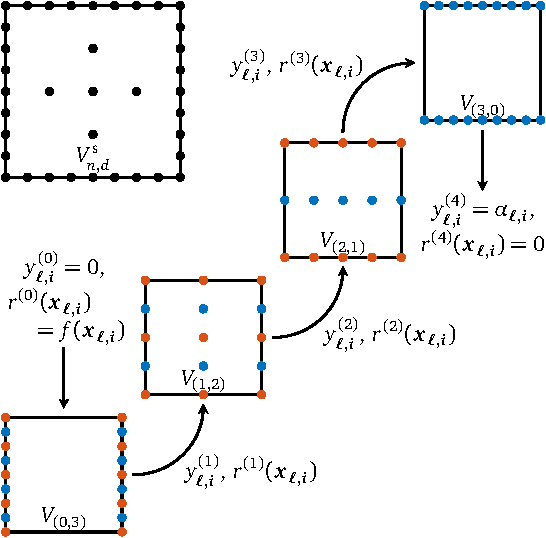
\includegraphics{residualInterpolation_1}%
  \caption[%
    Hierarchization with residual interpolation%
  ]{%
    Hierarchization of function value data on the
    two-dimensional regular sparse grid
    $\regsgspace{n}{d}$ of level $n = 3$ \emph{(top left)}
    using the method of residual interpolation.
    In this figure, we use
    $\linout[(j)]{\*l,\*i} \ceq \sum_{j'=1}^j \surplus[(j')]{\*l,\*i}$
    as an abbreviation.
    The order of the nodal spaces (here: bottom left to top right)
    does not matter.
    The data $\linout[(j)]{\*l,\*i}$
    corresponding to \textcolor{C0}{blue grid points}
    will not be modified in the remaining iterations
    and, therefore, already equals the correct surpluses $\surplus{\*l,\*i}$.
    The data corresponding to \textcolor{C1}{red grid points}
    will be modified as the grid points appear in one of the remaining
    nodal grids.%
  }%
  \label{fig:residualInterpolation}%
\end{SCfigure}

\longsection{%
  \texorpdfstring{%
    Hierarchization on Spatially Adaptive Sparse Grids\\
    with Breadth-First Search%
  }{%
    Hierarchization on Spatially Adaptive Sparse Grids
    with Breadth-First Search%
  }%
}{%
  Hierarchization on Spatially Adaptive Sparse Grids
  with Breadth-First Search%
}{%
  Hierarchization with Breadth-First Search%
}
\label{sec:44spatAdaptiveBFS}

\minitoc{87mm}{8}

\noindent
Unfortunately, we cannot apply the algorithms presented in the last
sections to spatially adaptive sparse grids with
hierarchical B-splines.
The reason is that the algorithms relied on the final interpolant $\sgintp$
being a linear combination of full grid solutions $\fgintp{\*l}$,
which is only possible for dimensionally adaptive sparse grids.
Consequently, the problem of hierarchization becomes significantly
harder if we operate on spatially adaptive sparse grids.
An exception is the case of piecewise linear basis functions ($p = 1$),
where we are still able to apply the \up,
as we will show in \cref{sec:45spatAdaptiveUP}.
%
In this section, we study one approach to hierarchize on
spatially adaptive sparse grids,
namely transforming the hierarchical basis to so-called fundamental bases
to enable a \bfs algorithm for hierarchization.

The approach in this section has already been published
\cite{Valentin18Fundamental}.
Again, note that while B-splines are our target application,
the considerations in this chapter are fully independent of the choice of
basis functions $\basis{\*l,\*i}$,
as long as they have tensor product structure.
Although we do not state it explicitly, it is possible to employ
different types of basis functions $\basis{l_t,i_t}$ in different
dimensions, e.g., B-splines of different degrees $p_t$
to enable $p$-adaptivity.



\fillsubsectionornament
\subsection{Hierarchization with Breadth-First Search on Fundamental Bases}
\label{sec:441BFSFundamentalBases}

\paragraph{Fundamental property}

As already discussed in \cref{sec:41problem},
the main cause of the difficulty of the hierarchization with B-splines
$\bspl{\*l,\*i}{p}$ is their overlapping support
(which they need for their approximation order).
Thus, high-level B-splines $\bspl{\*l',\*i'}{p}$ do not vanish
at all coarse-level grid points $\gp{\*l,\*i}$, $\*l < \*l'$.
In the univariate case,
\pagebreak%
the idea is to transform the B-spline basis to obtain
new basis functions $\fundbasis{l',i'}\colon \clint{0, 1} \to \real$
($l' \in \natz$, $i' \in \hiset{l'}$) that satisfy
\begin{subequations}
  \label{eq:fundamentalProperty}
  \begin{alignat}{3}
    \label{eq:fundamentalProperty1}
    \fundbasis{l',i'}(\centerhphantom{\gp{l,i}}{\gp{l',i}})
    &= 0,\qquad
    &&l < l',\quad
    &&i \in \hiset{l},\\
    \label{eq:fundamentalProperty2}
    \fundbasis{l',i'}(\gp{l',i})
    &= \kronecker{i}{i'},\qquad
    &&&&i \in \hiset{l'}.
  \end{alignat}
\end{subequations}
We call \eqref{eq:fundamentalProperty} \term{fundamental property}
and functions $\fundbasis{l',i'}$
that fulfill this property \term{fundamental basis functions.}
The first \cref{eq:fundamentalProperty1} ensures that
basis functions of level $l'$ vanish at
grid points of coarser levels $l < l'$.
The second \cref{eq:fundamentalProperty2} requires the
basis functions $\fundbasis{l',i'}$
to additionally vanish at all grid points of the same level $l'$
with different index $i \not= i'$.
An example for fundamental basis functions are
the piecewise linear B-splines $\bspl{l',i'}{1}$
or the Lagrange polynomials $\lagrangepoly{l',i'}$
(see \cref{fig:fundamentalProperty}, left).
The statement that $\fundbasis{l',i'}(\gp{l',i'})$ should equal one
is not an additional restriction, if
the value $\fundbasis{l',i'}(\gp{l',i'})$ is non-zero,
since we can just replace $\fundbasis{l',i'}$ with
$\fundbasis{l',i'}/\fundbasis{l',i'}(\gp{l',i'})$ to obtain
$\fundbasis{l',i'}(\gp{l',i'}) = 1$.

\begin{SCfigure}
  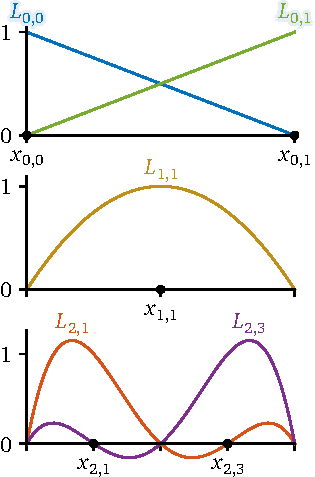
\includegraphics{hierarchicalBasis_13}\quad%
  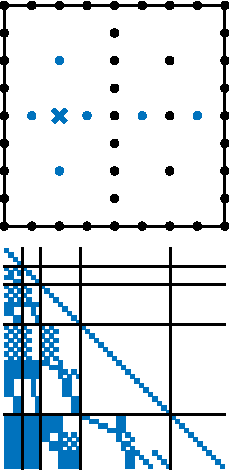
\includegraphics{matrixDensityPattern_2}%
  \caption[%
    Fundamental property with Lagrange polynomials as fundamental basis%
  ]{%
    Fundamental property with Lagrange polynomials.\\
    \emph{Left:}
    Univariate Lagrange polynomials up to level $l = 2$.\\
    \emph{Top right:}
    Regular sparse grid $\coarseregsgset{n}{d}{1}$
    ($n = 4$, $d = 2$).
    The fundamental basis function $\fundbasis{\*l',\*i'}$ corresponding
    to the marked grid point \emph{(cross)} does not vanish
    at the \textcolor{C0}{blue points} $\gp{\*l,\*i}$
    (which satisfy \eqref{eq:fundamentalPropertyImplicationMV}).\\
    \emph{Bottom right:}
    Corresponding density pattern of $\intpmat$
    when sorting rows and columns by increasing level sum
    $\normone{\*l} = 0, \dotsc, n$ \emph{(black bars).}%
  }%
  \label{fig:fundamentalProperty}%
\end{SCfigure}

\paragraph{Multivariate case}

For the multivariate case of $d \in \nat$ dimensions,
we define as usual tensor product versions
$\fundbasis{\*l',\*i'}$ of the univariate fundamental bases
$\fundbasis{l'_t,i'_t}$ ($t = 1, \dotsc, d$).
\Cref{eq:fundamentalProperty} then implies
\begin{equation}
  \label{eq:fundamentalPropertyImplicationMV}
  \fundbasis{\*l',\*i'}(\gp{\*l,\*i}) \not= 0
  \implies
  \falarge{t = 1, \dotsc, d}{
    \bracket*{(l'_t < l_t) \lor ((l'_t, i'_t) = (l_t, i_t))}
  },\quad
  (\*l, \*i), (\*l',\*i') \in \liset.
  \hspace*{-1mm}
\end{equation}
This means that every basis function
$\fundbasis{\*l',\*i'}$ can only be non-zero
at the grid points $\gp{\*l,\*i}$ that, in every dimension $t$,
have a strictly higher level $l_t$ or
the same level-index pair $(l_t, i_t)$ as the basis function.
We show an example for this relation in
\cref{fig:fundamentalProperty} (top right).

\paragraph{Triangular interpolation matrix}

The main motivation for enforcing the fundamental property
is the fact that it results in the hierarchization matrix $\intpmat$
being triangular, if the rows and columns are arranged
in the order of monotonously increasing level sum:
We assume that $k = k(\*l, \*i) \in \{1, \dotsc, N\}$ is a single
continuously enumerated index of the level-index pairs $(\*l, \*i) \in \liset$
(where $N = \setsize{\liset}$) such that
\begin{equation}
  k(\*l, \*i) \le k(\*l', \*i') \implies \normone{\*l} \le \normone{\*l'},\quad
  (\*l, \*i), (\*l', \*i') \in K,
\end{equation}
i.e., we sort the row indices $k = k(\*l, \*i)$ and
the column indices $k' = k(\*l', \*i')$ of $\intpmat$
by level sum $\normone{\cdot}$.
Consequently,
$\intpmat = (\intpmatentry{k}{k'})_{k=1,\dotsc,N,\, k'=1,\dotsc,N}$
is in lower block-triangular form:
\begin{subequations}
  \label{eq:fundamentalTriangularMV}
  \begin{alignat}{2}
    \intpmatentry{k}{k'}
    &= \fundbasis{k'}(\vgp{k})
    = 0,\quad
    &\normone{\*l}
    &< \normone{\*l'},\\
    \intertext{%
      as $\normone{\*l} < \normone{\*l'} \implies \ex{t}{l_t < l'_t}$
      and using \eqref{eq:fundamentalProperty1}.
      Additionally, the diagonal blocks are unit matrices due to%
    }
    \intpmatentry{k}{k'}
    &= \fundbasis{k'}(\vgp{k})
    \overset{(\ast)}{=} \kronecker{(\*l,\*i)}{(\*l',\*i')},\quad
    &\normone{\*l}
    &= \normone{\*l'},
  \end{alignat}
\end{subequations}
since $\normone{\*l} = \normone{\*l'}$ implies that
either $\bracket*{\ex{t}{l_t < l'_t}}$ or $\*l = \*l'$.%
\footnote{%
  Note that as specified in the list of symbols at the beginning
  of this thesis, the Kronecker delta $\kronecker{X}{Y}$
  is defined for arbitrary objects $X$ and $Y$
  that can be compared with ``$=$.''%
}
In the former case, both sides of $(\ast)$ vanish
(according to \eqref{eq:fundamentalProperty1}),
and in the latter case,
both sides equal $\kronecker{\*i}{\*i'}$
(according to \eqref{eq:fundamentalProperty2}).
Hence, $\intpmat$ is a lower-triangular matrix.
This is visualized for a two-dimensional example in
\cref{fig:fundamentalProperty} (bottom right).

\paragraph{Forward substitution}

The triangular structure of $\intpmat$ implies that
we can determine the surpluses $\surplus{\*l,\*i}$
via forward substitution:

\begin{lemma}[forward substitution]
  \label{lemma:forwardSubstitution}
  The hierarchical surpluses $\surplus{\*l,\*i}$, which
  are determined by \eqref{eq:hierarchizationSLE}
  with respect to $\fundbasis{\*l,\*i}$, satisfy
  \begin{equation}
    \surplus{\*l,\*i}
    = \fcnval{\*l,\*i} -
    \largesum{\substack{(\*l',\*i')\in\liset\\\normone{\*l'} < \normone{\*l}}}
    \surplus{\*l',\*i'} \fundbasis{\*l',\*i'}(\gp{\*l,\*i}),\quad
    (\*l, \*i) \in \liset.
  \end{equation}
\end{lemma}

\begin{proof}
  The linear system \eqref{eq:hierarchizationSLE} is given by
  \begin{subequations}
    \setlength{\abovedisplayskip}{9pt}%
    \setlength{\belowdisplayskip}{9pt}%
    \begin{align}
      \fcnval{\*l,\*i}
      &= \largesum{(\*l',\*i') \in \liset}
      \surplus{\*l',\*i'} \fundbasis{\*l',\*i'}(\gp{\*l,\*i}),\quad
      (\*l, \*i) \in \liset.\\
      \intertext{%
        According to \eqref{eq:fundamentalTriangularMV},
        all summands with $\normone{\*l'} > \normone{\*l}$ vanish
        and from the summands with $\normone{\*l'} = \normone{\*l}$,
        only the $(\*l, \*i)$-th summand remains
        with $\fundbasis{\*l,\*i}(\gp{\*l,\*i}) = 1$:%
      }
      \cdots
      &= \surplus{\*l,\*i} +
      \largesum{\substack{(\*l',\*i')\in\liset\\\normone{\*l'} < \normone{\*l}}}
      \surplus{\*l',\*i'} \fundbasis{\*l',\*i'}(\gp{\*l,\*i}).\\[-6.4em]\notag
    \end{align}
  \end{subequations}
\end{proof}

\vspace{1em}

\paragraph{Breadth-first search}

Exploiting this lemma, we formulate
a hierarchization algorithm (see \cref{alg:BFS})
that applies forward substitution by \bfs in the \dagr of
the spatially adaptive sparse grid $\sgset$.
The nodes of the \dagr are the level-index pairs $(\*l, \*i) \in \liset$.
An edge connects $(\*l, \*i)$ to $(\*l', \*i')$,
if $(\*l, \*i)$ is a direct ancestor of $(\*l', \*i')$, i.e., if
{%
  \setlength{\abovedisplayskip}{9pt}%
  \setlength{\belowdisplayskip}{9pt}%
  \begin{equation}
    \label{eq:directAncestor}
    \exlarge{t = 1, \dotsc, d}{
      \*l'_{-t} = \*l^{}_{-t},\;
      \*i'_{-t} = \*i^{}_{-t},\;
      l'_t = l^{}_t + 1,\;
      i'_t \in
      \begin{cases}
        \{1\},&l_t = 0,\\
        \{2i_t - 1, 2i_t + 1\},&l_t > 0.
      \end{cases}
    }
  \end{equation}%
}%
An example for the resulting \dagr for a regular sparse grid
in two dimensions is shown in \cref{fig:DAG}.
%
\begin{algorithm}
  \begin{algorithmic}[1]
    \Function{$\vlinout = \texttt{breadthFirstSearch}$}{%
      $\vlinin$, $\liset$%
    }
      \State{$\vlinout \gets \vlinin$}
      \label{line:algBFS3}
      \State{$K_\mathrm{p} \gets \{\*0\} \times \{0, 1\}^d$}
      \Comment{set of processed points}%
      \State{%
        $Q \gets \text{FIFO queue initialized with contents of } K_\mathrm{p}$%
      }
      \Comment{points to be processed}%
      \While{$Q \not= \emptyset$}
        \State{$(\*l', \*i') \gets Q.\pop()$}
        \Comment{obtain next point}%
        \For{%
          $\{(\*l, \*i) \in \liset \setminus \{(\*l', \*i')\} \mid
          \fa{t=1,\dotsc,d}{(l'_t < l_t) \lor ((l'_t, i'_t) = (l_t, i_t))}\}$%
        }
        \label{line:algBFS1}
          \State{%
            $\linout{\*l,\*i} \gets \linout{\*l,\*i} -
            \linout{\*l',\*i'} \fundbasis{\*l',\*i'}(\gp{\*l,\*i})$%
          }
          \Comment{%
            update surpluses according to \cref{lemma:forwardSubstitution}%
          }%
          \label{line:algBFS2}
        \EndFor{}
        \For{%
          $\{(\*l, \*i) \in \liset \setminus \liset_\mathrm{p} \mid
          \text{$(\*l, \*i)$ direct child of $(\*l', \*i')$}\}$%
        }
          \State{$Q.\push((\*l, \*i))$}
          \Comment{add children to queue}%
          \State{%
            $\liset_\mathrm{p} \gets
            \liset_\mathrm{p} \cup \{(\*l, \*i)\}$%
          }
          \Comment{mark as processed}%
        \EndFor{}
      \EndWhile{}
    \EndFunction{}
  \end{algorithmic}
  \caption[%
    Hierarchization with breadth-first search (BFS)%
  ]{%
    Hierarchization with breadth-first search
    on spatially adaptive sparse grids with fundamental bases.
    Inputs are
    the vector $\vlinin = (\linin{\*l,\*i})_{(\*l,\*i) \in \liset}$
    of input data (function values $\fcnval{\*l,\*i}$ at the grid points) and
    the set $\liset$ of level-index pairs of the
    sparse grid (see \eqref{eq:spatiallyAdaptiveSG}).
    The output is the vector
    $\vlinout = (\linout{\*l,\*i})_{(\*l,\*i) \in \liset}$
    of output data (hierarchical surpluses $\surplus{\*l,\*i}$).%
  }%
  \label{alg:BFS}%
\end{algorithm}
%
\begin{SCfigure}
  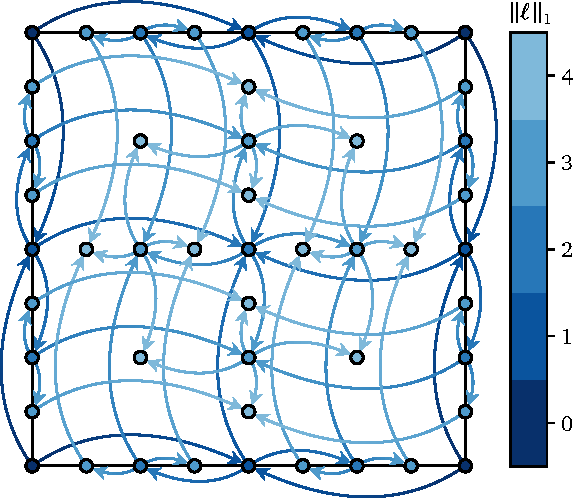
\includegraphics{dag_1}%
  \caption[%
    Sparse grid as directed acyclic graph%
  ]{%
    Ancestor relationships \emph{(arrows)} in a
    regular sparse grid $\coarseregsgset{n}{d}{1}$ \emph{(points)}
    of level $n = 4$ and dimensionality $d = 2$.
    The color indicates the level sum $\normone{\*l}$.
    Breadth-first search, as implemented in \cref{alg:BFS},
    visits all grid points $\gp{\*l,\*i}$ with level sum
    $\normone{\*l} = 0$ first,
    then those with $\normone{\*l} = 1$, and so on.%
  }%
  \label{fig:DAG}%
\end{SCfigure}
%
We make two assumptions for \cref{alg:BFS}.
First, $\liset$ should contain at least all $2^d$ corners of the
domain $\clint{\*0, \*1}$:
\begin{subequations}
  \label{eq:BFSAssumptions}
  \begin{equation}
    \label{eq:BFSAssumption1}
    \liset \supset \{\*0\} \times \{0, 1\}^d
    = \{(\*0, \*i) \mid \*i \in \{0, 1\}^d\}.
  \end{equation}
  Second, all grid points should be reachable from the corners:
  \begin{equation}
    \label{eq:bfsAssumption2}
    \begin{split}
      \forall_{(\*l', \*i') \in \liset}
      \exists_{m \in \natz}
      \exists_{
        (\*l^{(0)}, \*i^{(0)}), \dotsc, (\*l^{(m)}, \*i^{(m)}) \in \liset
      }\;\;
      &\bigl[(\*l^{(0)}, \*i^{(0)}) \to \dotsb \to (\*l^{(m)}, \*i^{(m)}),\\
      &\hspace{3mm} \*l^{(0)} = \*0,\;
      (\*l^{(m)}, \*i^{(m)}) = (\*l', \*i')\bigr],
    \end{split}
  \end{equation}
\end{subequations}
where ``$\to$'' is the direct ancestor relation \eqref{eq:directAncestor}.
One can also use a different initial set than the corners
of $\clint{\*0, \*1}$, e.g., when working with sparse grids
without boundary points.
In general, there are three requirements on the initial set:
First, all grid points should be reachable from this set.
Second, the grid points in the set are sorted by increasing level sum
(if the set contains grid points with different level sums).
Third, the surpluses corresponding to the initial grid points
need to be precalculated correctly
before the \texttt{\algorithmicwhile} loop in \cref{alg:BFS}.

\paragraph{Correctness}

The correctness of \cref{alg:BFS} can be shown with the following invariant:

\begin{restatable}[invariant of breadth-first-search hierarchization]{%
  proposition%
}{%
  propInvariantBFS%
}
  \label{prop:invariantBFS}
  Under the assumption \eqref{eq:BFSAssumptions},
  it holds after \pop{}\,ping all grid points with level sum $< q$
  from the queue $Q$ in \cref{alg:BFS}:
  \begin{equation}
    \label{eq:propInvariantBFS}
    \linout{\*l,\*i}
    = \fcnval{\*l,\*i} -
    \largesum{\substack{(\*l',\*i')\in\liset\\\normone{\*l'} < q}}
    \linout{\*l',\*i'} \fundbasis{\*l',\*i'}(\gp{\*l,\*i}),\quad
    (\*l, \*i) \in \liset,\;\;
    \normone{\*l} = q.
    \hspace*{-6mm}
  \end{equation}
\end{restatable}

\vspace{-0.8em}

\begin{proof}
  See \cref{sec:a133proofBFS}.
\end{proof}

\vspace{0.8em}

\begin{shortcorollary}[correctness of breadth-first-search hierarchization]
  \label{cor:algBFSCorrectness}
  \Cref{alg:BFS} is correct.
\end{shortcorollary}

\begin{proof}
  As noted in the proof of \cref{prop:invariantBFS},
  the result $\linout{\*l,\*i}$ after \pop{}ping all grid points with level sum
  $q$ as stated in \cref{prop:invariantBFS} is also the final result
  of the algorithm:
  \begin{equation}
    \linout{\*l,\*i}
    = \fcnval{\*l,\*i} -
    \largesum{\substack{(\*l',\*i')\in\liset\\\normone{\*l'} < \normone{\*l}}}
    \linout{\*l',\*i'} \fundbasis{\*l',\*i'}(\gp{\*l,\*i}),\quad
    (\*l, \*i) \in \liset.
  \end{equation}
  By \cref{lemma:forwardSubstitution},
  the correct hierarchical surpluses $\surplus{\*l,\*i}$
  satisfy the same relation.
  Inductively, $\linout{\*l,\*i}$ and $\surplus{\*l,\*i}$ must coincide.
\end{proof}

\paragraph{Complexity}

The \bfs algorithm in \cref{alg:BFS} is not as efficient as the \up:
It still needs to perform $\landauO{N^2 d}$ many univariate
basis evaluations (compared to $\landauO{Nd}$ for the \up).
However, it only needs linear space $\landauO{N}$ similar to the
\up\punctfix{.}
This is a significant advantage over directly solving the system
\eqref{eq:hierarchizationSLE} of linear equations, which typically
needs quadratic space $\landauO{N^2}$.



\subsection{Constructing Fundamental Bases}
\label{sec:442constructingFundamentalBases}

Unfortunately, the hierarchical B-splines $\bspl{l',i'}{p}$ do not
satisfy the fundamental property \eqref{eq:fundamentalProperty}.
We now focus on the construction of univariate fundamental bases
$\fundbasis{l',i'}$ starting from an
arbitrary hierarchical basis $\basis{l',i'}$.
To this end, we study two transformations
$\basis{l',i'} \mapsto \fundbasis{l',i'}$.
As usual, the multivariate case is treated with the
tensor product approach.

\paragraph{Hierarchical fundamental transformation (HFT)}

The canonical way to find a fundamental basis $\fundbasis{l',i'}$ is to
use a linear combination $\basis[\hft]{l',i'}$
of coarser basis functions $\basis{l'',i''}$ as an ansatz
and require that the fundamental property \eqref{eq:fundamentalProperty}
is fulfilled:
\begin{equation}
  \label{eq:hierarchicalFundamentalTransformation}
  \basis[\hft]{l',i'}
  \ceq \sum_{l''=0}^{l'} \sum_{i'' \in \hiset{l''}}
  c_{l'',i''}^{l',i'} \basis{l'',i''}
  \quad\text{such that}\quad
  \fafalarge{l = 0, \dotsc, l'}{i \in \hiset{l}}{
    \basis[\hft]{l',i'}(\gp{l,i}) = \kronecker{(l,i)}{(l',i')}.
  }
\end{equation}
This means that
$\basis[\hft]{l',i'}$ ($l' \in \natz$, $i' = 0, \dotsc, 2^{l'}$)
interpolates the data
$\{(\gp{l',i}, \kronecker{i}{i'}) \mid i = 0, \dotsc, 2^{l'}\}$.
The coefficients $c_{l'',i''}^{l',i'} \in \real$
are, in general, different for each basis function $\basis[\hft]{l',i'}$.
This complicates precomputation and storage of the $2^{l'} + 1$ coefficients,
as they have to be determined by solving a system of linear equations.
In addition, the transformation $\basis{l',i'} \mapsto \basis[\hft]{l',i'}$
does not preserve the locality of the support of the basis functions.
Consequently, $\basis[\hft]{l',i'}$ may be globally supported,
which means that we have to evaluate up to $2^{l'} + 1$ basis functions
$\basis{l'',i''}$ when evaluating $\basis[\hft]{l',i'}$ at a single point
$x \in \clint{0, 1}$.
The global support of the resulting transformed basis
for uniform hierarchical B-splines (which are locally supported)
can be seen in \cref{fig:hftBSpline}.

\begin{SCfigure}
  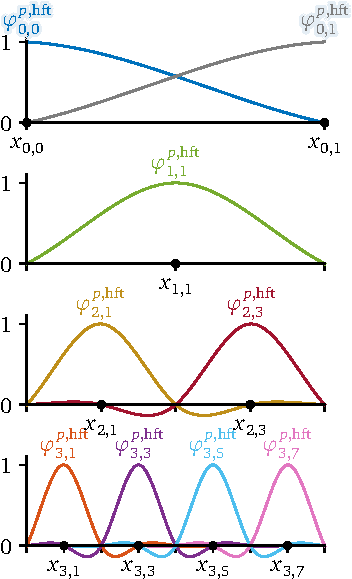
\includegraphics{hierarchicalBasis_14}%
  \caption[%
    Hierarchical fundamental transformation on hierarchical B-splines%
  ]{%
    Resulting basis functions $\bspl[\hft]{l',i'}{p}$
    ($l' \le l$, $i' \in \hiset{l'}$)
    after applying the hierarchical fundamental transformation
    to hierarchical cubic B-splines ($p = 3$) and
    grid points $\gp{l',i'}$ \emph{(dots)} up to level $l = 3$.%
  }%
  \label{fig:hftBSpline}%
\end{SCfigure}

We call the transformation $\basis{l',i'} \mapsto \basis[\hft]{l',i'}$
\term{\hftr.}
The following proposition shows that this is only a change of basis,
as the spanned sparse grid space remains unchanged.
While the proposition is formulated for regular sparse grids,
a similar statement can be proven for the dimensionally adaptive case.

\begin{proposition}[%
  spanned sparse grid space for the HFT%
]
  \label{prop:hftSparseGridSpace}
  If $\liset \ceq \{(\*l, \*i) \mid
  \normone{\*l'} \le n,\; \*i' \in \hiset{\*l'}\}$
  is the set of level-index pairs for the regular sparse grid of level $n$
  and dimensionality $d$, then
  \begin{equation}
    \regsgspace{n}{d}
    = \regsgspace[\hft]{n}{d}
    \ceq \spn\{\basis[\hft]{\*l',\*i'} \mid (\*l', \*i') \in \liset\}.
  \end{equation}
\end{proposition}

\begin{proof}
  We have $\regsgspace{n}{d} \supset \regsgspace[\hft]{n}{d}$ as
  $\basis[\hft]{\*l',\*i'} \in \regsgspace{n}{d}$
  for all $(\*l', \*i') \in \liset$:
  \begin{equation}
    \basis[\hft]{\*l',\*i'}
    = \prod_{t=1}^d \, \sum_{l''_t=0}^{l'_t} \, \sum_{i''_t \in \hiset{l''_t}}
    c_{l''_t,i''_t}^{l'_t,i'_t} \basis{l''_t,i''_t}
    = \sum_{\*l''=\*0}^{\*l'} \, \sum_{\*i'' \in \hiset{\*l''}}
    c_{\*l'',\*i''}^{\*l',\*i'} \basis{\*l'',\*i''}
    \in \regsgspace{n}{d},\quad
    c_{\*l'',\*i''}^{\*l',\*i'}
    \ceq \prod_{t=1}^d c_{l''_t,i''_t}^{l'_t,i'_t}.
  \end{equation}
  
  To prove that $\regsgspace{n}{d} \subset \regsgspace[\hft]{n}{d}$,
  we show that the dimension of $\regsgspace[\hft]{n}{d}$
  matches $\dim \regsgspace{n}{d} = \setsize{\liset}$.
  It suffices to show that
  the functions $\basis[\hft]{\*l',\*i'}$ ($(\*l', \*i') \in \liset$),
  are linearly independent.
  Let $\surplus{\*l',\*i'} \in \real$ be with
  $\sum_{(\*l', \*i') \in \liset}
  \surplus{\*l',\*i'} \basis[\hft]{\*l',\*i'} \equiv 0$.
  By evaluating at $\gp{\*l,\*i}$ ($(\*l, \*i) \in \liset$), we obtain
  \begin{equation}
    \largesum{(\*l', \*i') \in \liset}
    \surplus{\*l',\*i'} \basis[\hft]{\*l',\*i'}(\gp{\*l,\*i}) = 0,\quad
    (\*l, \*i) \in \liset.
  \end{equation}
  This is a lower triangular system according to
  \eqref{eq:fundamentalTriangularMV},
  which implies $\surplus{\*l',\*i'} = 0$ for all $(\*l, \*i) \in \liset$.
  Hence, the functions $\basis[\hft]{\*l',\*i'}$ ($(\*l', \*i') \in \liset$)
  are linearly independent.
\end{proof}

\paragraph{Translation-invariant fundamental transformation (TIFT)}

Another disadvantage of the \hftr is that it does not preserve
the so-called \term{translation invariance} of the original basis.
A~basis $\basis{l,i}$ ($l \in \natz$, $i = 0, \dotsc, 2^l$)
is translation-invariant, if there is a \term{parent function}
$\parentfcn\colon \real \to \real$
such that
\begin{equation}
  \label{eq:translationInvariance}
  \basis{l,i}(x)
  = \parentfcn(\tfrac{x}{\ms{l}} - i),\quad
  l \in \natz,\;\;
  i = 0, \dotsc, 2^l,\;\;
  x \in \clint{0, 1}.
\end{equation}
The fact that the \hftr does not preserve translation invariance means
that for each basis function $\basis[\hft]{l',i'}$, we have to
calculate its individual $2^{l'} + 1$ coefficients $c_{l'',i''}^{l',i'}$.

To solve this problem,
we use a similar ansatz as for the \hftr,
but we replace the hierarchical basis functions $\basis{l'',i''}$
($l'' = 0, \dotsc, l'$,\, $i'' \in \hiset{l''}$)
with nodal basis functions $\basis{l',i''}$ and
allow general integer indices $i'' \in \integer$:
\begin{equation}
  \label{eq:tiftDefinition}
  \basis[\tift]{l',i'}
  \ceq \sum_{i'' \in \integer} c_{i''}^{l',i'} \basis{l',i''}
  \quad\text{such that}\quad
  \falarge{i \in \hiset{l'}}{
    \basis[\tift]{l',i'}(\gp{l',i}) = \kronecker{i}{i'},
  }
\end{equation}
where $l' \in \natz$, $i' = 0, \dotsc, 2^{l'}$, and
$c_{i''}^{l',i'} \in \real$.
We have to make three assumptions for \eqref{eq:tiftDefinition} to make sense:

\begin{itemize}
  \item
  The functions $\basis{l',i''}$ have to be defined for integer indices
  $i'' \in \integer$, i.e.,
  the functions $\basis{l',i''}\colon \clint{0, 1} \to \real$
  must also exist for $i'' < 0$ or $i'' > 2^{l'}$.
  This is the case for translation-invariant bases
  $\basis{l',i''}$ (such as B-splines $\bspl{l',i''}{p}$),
  as they can be generalized to $i'' \in \integer$
  via \cref{eq:translationInvariance}.
  
  \item
  The set
  \begin{equation}
    \relindexset{l'}
    \ceq \braced*{
      i'' \in \integer \bigm\vert
      \restrictfcn{\basis{l',i''}}{\clint{0, 1}} \not\equiv 0
    },\quad
    l' \in \natz,
  \end{equation}
  of relevant indices should be finite,
  so that in each point $x \in \clint{0, 1}$
  only a finite number of basis functions $\basis{l',i''}$ of level $l'$
  is non-zero.
  This means that the series in \eqref{eq:tiftDefinition} collapses to a
  finite sum over $i'' \in \relindexset{l'}$.
  The condition is met for compactly supported and translation-invariant
  basis functions such as B-splines $\bspl{l',i''}{p}$.
  For $d \in \nat$ dimensions and $\*l' \in \natz^d$, we define
  $\relindexset{\*l'} \ceq
  \relindexset{l'_1} \times \dotsb \times \relindexset{l'_d}$.
  
  \item
  The coefficients $c_{i''}^{l',i'}$, such that
  \eqref{eq:tiftDefinition} holds, exist and are uniquely determined.
\end{itemize}

\vspace{1em}

\noindent
Let $\basis{l',i''}$ be translation-invariant and
let $l' \in \natz$ and $i' = 0, \dotsc, 2^{l'}$ be arbitrary.
Then we have
\begin{equation}
  \label{eq:tiftParentFunctionDerivation}
  \basis[\tift]{l',i'}(x)
  = \sum_{i'' \in \integer} c_{i''}^{l',i'} \basis{l',i''}(x)
  \!\overset{\eqref{eq:translationInvariance}}{=}\!
  \sum_{i'' \in \integer} c_{i''}^{l',i'}
  \parentfcn(\tfrac{x}{\ms{l'}} - i'')
  = \sum_{i'' \in \integer}
  c_{i'+i''}^{l',i'} \parentfcn((\tfrac{x}{\ms{l'}} - i') - i''),
\end{equation}
where the function defined by
$\sum_{i'' \in \integer} c_{i'+i''}^{l',i'} \parentfcn({\cdot} - i'')$
satisfies
\begin{subequations}
  \label{eq:tiftParentFunctionConditions}
  \begin{align}
    \sum_{i'' \in \integer} c_{i'+i''}^{l',i'} \parentfcn(i - i'')
    &= \sum_{i'' \in \integer} c_{i'+i''}^{l',i'}
    \parentfcn((\tfrac{\gp{l',i+i'}}{\ms{l'}} - i') - i'')
    \!\overset{\eqref{eq:tiftParentFunctionDerivation}}{=}\!
    \basis[\tift]{l',i'}(\gp{l',i+i'})
    \!\overset{\eqref{eq:tiftDefinition}}{=}\!
    \kronecker{i'}{i+i'}\\
    &= \kronecker{i}{0},\quad
    i \in \integer.
  \end{align}
\end{subequations}
Due to the translation invariance and the third assumption in the list above,
there is only a single set of coefficients of $\parentfcn({\cdot} - i'')$
such that \eqref{eq:tiftParentFunctionConditions} holds.
This means that $c_{i'+i''}^{l',i'}$ does not depend on $l'$ or $i'$,
if $\basis{l',i'}$ is translation-invariant.
Consequently, if we set $c_{i''} \ceq c_{i'+i''}^{l',i'}$
for some arbitrary $l' \in \natz$ and $i' = 0, \dotsc, 2^{l'}$,
then $\parentfcn[\tift]\colon \real \to \real$ defined by
\begin{equation}
  \label{eq:tiftParentFunctionDefinition}
  \parentfcn[\tift](x)
  \ceq \sum_{i'' \in \integer} c_{i''} \parentfcn(x - i''),\quad
  x \in \clint{0, 1},
\end{equation}
is a parent function of $\basis[\tift]{l',i'}$ that satisfies
\begin{equation}
  \label{eq:tiftParentFunctionInterpolation}
  \falarge{i \in \integer}{
    \parentfcn[\tift](i) = \kronecker{i}{0}.
  }
\end{equation}
The fact that $\parentfcn[\tift]$ is the parent function of
$\basis[\tift]{l',i'}$ easily follows from
\eqref{eq:tiftParentFunctionDerivation}
as the \rhs is exactly $\parentfcn[\tift](\tfrac{x}{\ms{l'}} - i')$,
as required by \eqref{eq:translationInvariance}.
This shows that the transformation $\basis{l',i'} \mapsto \basis[\tift]{l',i'}$
preserves translation-invariance.
Therefore, we call the transformation
$\basis{l',i'} \mapsto \basis[\tift]{l',i'}$ \term{\tiftr.}

\vspace{2em}

In contrast to the \hftr, the \tiftr is only a change of basis
if we consider the extended nodal spaces that also include
basis functions with indices outside $\{0, \dotsc, 2^{l'}\}$.
This is the statement of the following proposition
(generalized to the $d$-variate case).
Note that although the proposition involves basis functions
$\basis{\*l',\*i'}$ and $\basis[\tift]{\*l',\*i'}$
outside the domain $\clint{0, 1}$
(in the sense that $\gp{\*l',\*i'} \notin \clint{0, 1}$),
we still restrict all functions to $\clint{0, 1}$.
We cannot formulate an equivalent version of \thmref{prop:hftSparseGridSpace},
as it might be that, in one dimension,
$\basis{l',i''}$ ($i'' < 0$ or $i'' > 2^{l'}$)
is not contained in the nodal space $\ns{l'}$.

\pagebreak

\begin{proposition}[%
  spanned nodal space for the TIFT%
]
  \label{prop:tiftNodalSpace}
  We have
  \begin{equation}
    \hspace*{-10mm}
    \spn\{\basis{\*l',\*i'} \mid \*i' \in \relindexset{\*l'}\}
    =: \ns[\ext]{\*l'}
    = \ns[\tift,\ext]{\*l'}
    \ceq \spn\{\basis[\tift]{\*l',\*i'} \mid \*i' \in \relindexset{\*l'}\},\quad
    \*l' \in \natz^d.
    \hspace*{-20mm}
  \end{equation}
\end{proposition}

\vspace{1em}

\begin{proof}
  We have $\ns[\ext]{\*l'} \supset \ns[\tift,\ext]{\*l'}$ as
  $\basis[\tift]{\*l',\*i'} \in \ns[\ext]{\*l'}$
  for all $\*i' \in \relindexset{\*l'}$:
  \begin{equation}
    \basis[\tift]{\*l',\*i'}
    = \prod_{t=1}^d \sum_{i''_t \in \relindexset{l'_t}}
    c_{i''_t}^{l'_t,i'_t} \basis{l'_t,i''_t}
    = \sum_{\*i'' \in \relindexset{\*l'}}
    c_{\*i''}^{\*l',\*i'} \basis{\*l',\*i''}
    \in \ns[\ext]{\*l'},\quad
    c_{\*i''}^{\*l',\*i'}
    \ceq \prod_{t=1}^d c_{i''_t}^{l'_t,i'_t}.
  \end{equation}
  
  To prove that
  $\ns[\ext]{\*l'} \subset \ns[\tift,\ext]{\*l'}$,
  we show that the dimensions of the two spaces match.
  As before, it suffices to show that
  the functions $\basis[\tift]{\*l',\*i'}$ ($\*i' \in \relindexset{\*l'}$)
  are linearly independent.
  Let $\surplus{\*l',\*i'} \in \real$ be with
  $\sum_{\*i' \in \relindexset{\*l'}}
  \surplus{\*l',\*i'} \basis[\tift]{\*l',\*i'} \equiv 0$.
  By evaluating at $\gp{\*l',\*i}$ ($\*i \in \relindexset{\*l'}$), we obtain
  \begin{equation}
    0
    = \sum_{\*i' \in \relindexset{\*l'}} \surplus{\*l',\*i'}
    \underbrace{\basis[\tift]{\*l',\*i'}(\gp{\*l',\*i})}_{=\kronecker{\*i}{\*i'}}
    = \surplus{\*l',\*i},\quad
    \*i \in \relindexset{\*l'},
  \end{equation}
  i.e., all coefficients $\surplus{\*l',\*i'}$ must vanish.%
  \footnote{%
    Note that we have to allow evaluations outside the
    domain $\clint{0, 1}$ for this step.
    However, this is feasible for proving the linear independence
    of $\basis[\tift]{\*l',\*i'}$, since we can just restrict the functions
    after showing that the extended nodal spaces equal.%
  }
  Hence, the functions $\basis[\tift]{\*l',\*i'}$ ($\*i' \in \relindexset{\*l'}$)
  are linearly independent.
\end{proof}



\fillsubsectionornament
\subsection{Hierarchical Fundamental Splines}
\label{sec:443fundamentalSplines}

\paragraph{Definition}

We now apply the translation-invariant fundamental transformation
to hierarchical B-splines $\bspl{l,i}{p}$ of degree $p$.
The parent function $\parentbspl{p}\colon \real \to \real$ of B-splines
and the set $\relindexset[p]{l}$ of relevant indices for level $l \in \natz$
are given by
\begin{equation}
  \parentbspl{p}(x)
  \ceq \cardbspl{p}(x + \tfrac{p+1}{2}),\qquad
  \relindexset[p]{l}
  \ceq \{-\tfrac{p-1}{2},\;
  -\tfrac{p-1}{2} + 1,\;
  \dotsc,\;
  2^l + \tfrac{p-1}{2}\},
\end{equation}
respectively.
According to \eqref{eq:tiftParentFunctionInterpolation},
the coefficients $\fundsplcoeff{k}{p} \in \real$ of
the transformed parent function $\parentfcn[p,\tift]$
in \cref{eq:tiftParentFunctionDefinition} are determined by a
\pagebreak%
bi-infinite-dimensional system of linear equations:
\begin{equation}
  \label{eq:fundamentalSplineSLE}
  \newcommand*{\vala}{\cardbspl{p}(\tfrac{p+1}{2} - 2)}
  \newcommand*{\valb}{\cardbspl{p}(\tfrac{p+1}{2} - 1)}
  \newcommand*{\valc}{\cardbspl{p}(\tfrac{p+1}{2})}
  \newcommand*{\vald}{\cardbspl{p}(\tfrac{p+1}{2} + 1)}
  \newcommand*{\vale}{\cardbspl{p}(\tfrac{p+1}{2} + 2)}
  \newcommand*{\ddotsr}{\rotatebox{16}{$\ddots$}}
  \newcommand*{\raiseentry}[1]{\raisebox{0.3em}{$#1$}}
  \paren*{
    \begin{array}{%
      @{}>{\raggedright\arraybackslash$}m{14mm}<{$}@{}%
      *{3}{%
        @{}>{\centering\arraybackslash$}m{23mm}<{$}@{}%
      }%
      @{}>{\raggedleft\arraybackslash$}m{14mm}<{$}@{}%
    }
      \ddotsr&\ddotsr&\ddotsr&       &       \\
      \ddotsr&\valc  &\valb  &\vala  &       \\
      \ddotsr&\vald  &\valc  &\valb  &\ddotsr\\
             &\vale  &\vald  &\valc  &\ddotsr\\
             &       &\ddotsr&\ddotsr&\ddotsr
    \end{array}
  }
  \cdot
  \begin{pmatrix}
    \vphantom{\ddotsr}\raiseentry{\vdots}\\
    \vphantom{\ddotsr}\raiseentry{\fundsplcoeff{-1}{p}}\\
    \vphantom{\ddotsr}\raiseentry{\fundsplcoeff{0}{p}}\\
    \vphantom{\ddotsr}\raiseentry{\fundsplcoeff{1}{p}}\\
    \vphantom{\ddotsr}\raiseentry{\vdots}
  \end{pmatrix}
  =
  \begin{pmatrix}
    \vphantom{\ddotsr}\raiseentry{\vdots}\\
    \vphantom{\ddotsr}\raiseentry{0}\\
    \vphantom{\ddotsr}\raiseentry{1}\\
    \vphantom{\ddotsr}\raiseentry{0}\\
    \vphantom{\ddotsr}\raiseentry{\vdots}
  \end{pmatrix}.
\end{equation}
As in each row only $p$ entries are non-zero,
the system matrix is a symmetric banded Toeplitz matrix%
\footnote{%
  The entries $a_{k,j}$ of a Toeplitz matrix $\mat{A}$
  solely depend on $k - j$, i.e.,
  $a_{k,j} = c_{k-j}$ for some vector $\*c$.%
}.
One can show that the linear system \eqref{eq:fundamentalSplineSLE}
is uniquely solvable:

\begin{theorem}[unique existence of fundamental spline coefficients]
  \label{thm:fundamentalSplineExistence}
  \usenotation{zzzzfs}
  The system \eqref{eq:fundamentalSplineSLE} has a unique solution
  $(\fundsplcoeff{k}{p})_{k \in \integer}$ and the corresponding parent function
  $\parentfundspl{p}\colon \real \to \real$ defined by
  $\parentfundspl{p}(x) \ceq
  \sum_{k \in \integer} \fundsplcoeff{k}{p} \parentbspl{p}(x - k)$
  satisfies
  \begin{equation}
    \exfalarge{\beta_p, \gamma_p \in \posreal}{x \in \real}{
      \abs{\parentfundspl{p}(x)}
      \le \beta_p \cdot (\gamma_p)^{-\abs{x}}.
    }
  \end{equation}
\end{theorem}

\begin{proof}
  See Theorems 1 and 2 in \cite{Schoenberg72Cardinal}.
\end{proof}

The function $\parentfundspl{p}$ from \cref{thm:fundamentalSplineExistence}
is well-known as the \term{fundamental spline} of degree~$p$
\multicite{Schoenberg72Cardinal,Schoenberg73Cardinal}.
Applications of fundamental splines are interpolation and
the definition of spline wavelets \cite{Chui92Introduction}.
The fundamental splines $\parentfundspl{p}$ of low degrees $p$ and
their bounding functions $\beta_p \cdot (\gamma_p)^{-\abs{x}}$
are plotted in \cref{fig:fundamentalSpline}.

\begin{figure}
  \subcaptionbox{%
    $p = 1$%
  }[72mm]{%
    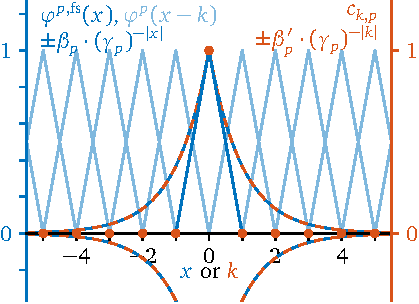
\includegraphics{fundamentalSpline_1}%
  }%
  \hfill%
  \subcaptionbox{%
    $p = 3$%
  }[72mm]{%
    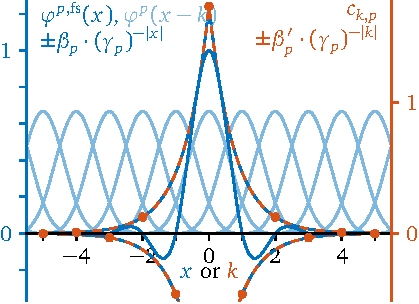
\includegraphics{fundamentalSpline_2}%
  }\\[4mm]%
  \subcaptionbox{%
    $p = 5$%
  }[72mm]{%
    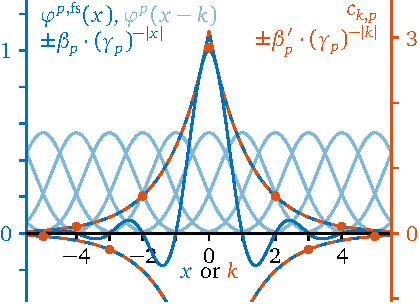
\includegraphics{fundamentalSpline_3}%
  }%
  \hfill%
  \subcaptionbox{%
    $p = 7$%
  }[72mm]{%
    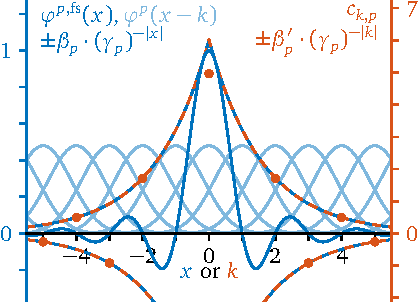
\includegraphics{fundamentalSpline_4}%
  }%
  \caption[%
    Fundamental splines and their B-spline coefficients%
  ]{%
    The fundamental spline $\parentfundspl{p}$ \emph{\textcolor{C0}{(blue)}}
    is a linear combination of cardinal B-splines $\cardbspl{p}({\cdot} - k)$,
    $k \in \integer$ \emph{\textcolor{C0!50}{(light blue)},}
    \vspace{-0.1em}%
    with coefficients $\fundsplcoeff{k}{p}$ \emph{\textcolor{C1}{(red points)}.}
    The absolute values of the fundamental spline $\parentfundspl{p}$ and
    its coefficients are bounded by a multiple of $(\gamma_p)^{-\abs{k}}$
    \emph{(\textcolor{C0}{blue}-\textcolor{C1}{red}-dashed line).}
    The axis for $\fundsplcoeff{k}{p}$ (on the right side) is scaled such that
    both bounding functions are on top of each other.%
  }%
  \label{fig:fundamentalSpline}%
\end{figure}

\paragraph{Definition of hierarchical fundamental splines}

The fundamental spline $\parentfundspl{p}$ defines
hierarchical fundamental spline functions
$\bspl[\fs]{l,i}{p}\colon \clint{0, 1} \to \real$ via
\cref{eq:translationInvariance}, i.e.,
\begin{equation}
  \bspl[\fs]{l,i}{p}(x)
  \ceq \parentfundspl{p}(\tfrac{x}{\ms{l}} - i),\quad
  l \in \natz,\;\;
  i = 0, \dotsc, 2^l,\;\;
  x \in \clint{0, 1}.
\end{equation}
The hierarchical cubic fundamental spline basis is depicted in
\cref{fig:hierarchicalFundamentalSpline}.
As usual, we define $d$-variate hierarchical fundamental splines
as tensor products of their univariate counterparts.
According to \thmref{prop:splineSpace} and \thmref{prop:tiftNodalSpace},
the common extended nodal space
$\nsbspl[\ext]{\*l}{\*p} = \nsbspl[\fs,\ext]{\*l}{\*p}$
is equal to the spline space $\wholesplspace{\*l}{\*p}$
defined by the Cartesian product of
knot sequences of the form \eqref{eq:fullGridKnots},
i.e., the space of all splines of degree $\*p$ on the full grid of level $\*l$.

\begin{SCfigure}
  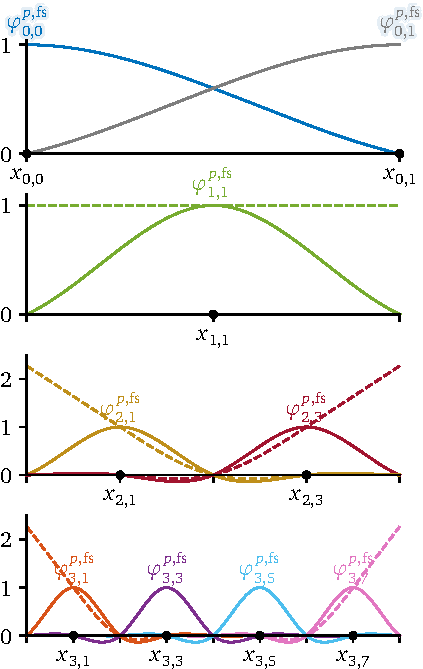
\includegraphics{hierarchicalBasis_15}%
  \caption[%
    Hierarchical fundamental splines%
  ]{%
    Hierarchical cubic fundamental splines
    $\bspl[\fs]{l',i'}{p}$
    ($l' \le l$, $i' \in \hiset{l'}$, $p = 3$),
    their modified versions $\bspl[\fs,\modified]{l',i'}{p}$
    \emph{(dashed),} and
    grid points $\gp{l',i'}$ \emph{(dots)} up to level $l = 3$.%
  }%
  \label{fig:hierarchicalFundamentalSpline}%
\end{SCfigure}

The B-spline coefficients $(\fundsplcoeff{k}{p})_{k \in \integer}$ of the
fundamental spline $\parentfundspl{p}$ decay with the same rate
as the fundamental spline itself due to the stability of the B-spline basis
\cite{Hoellig13Approximation}, i.e.,
\begin{equation}
  \label{eq:fundamentalSplineCoefficientsDecay}
  \abs{\fundsplcoeff{k}{p}}
  \le \beta'_p \cdot (\gamma_p)^{-\abs{k}},\quad
  k \in \integer,
\end{equation}
for some $\beta'_p > 0$ independent of $k$,
which is also shown in \cref{fig:fundamentalSpline}.
For $p > 1$,
there is a surprising relationship between the optimal (i.e., largest)
decay rate $\gamma_p$ and the polynomial
$\sum_{k=1}^p \cardbspl{p}(k) x^{k-1}$,
whose coefficients are the values of the
cardinal B-spline $\cardbspl{p}$ at its inner knots:
The decay rate is given by the absolute value of the largest root smaller
than $-1$ of said polynomial
(see \multicite{Chui92Introduction,Schoenberg73Cardinal}).

\vspace*{\fill}

Due to \eqref{eq:fundamentalSplineCoefficientsDecay},
we may solve the system \eqref{eq:fundamentalSplineSLE}
of linear equations approximately,
if we symmetrically truncate the linear system to
\pagebreak
$2\fundsplcutoff{p} - 1$ rows and columns
and set $\fundsplcoeff{k}{p} \ceq 0$ for all $\abs{k} \ge \fundsplcutoff{p}$,
where $\fundsplcutoff{p} \in \nat$ is a truncation index.
Note that we only have to perform $p + 1$ cardinal B-spline evaluations
to evaluate $\parentfundspl{p}$ once.
In \cref{tbl:fundamentalSplineDecay}, we list the decay rates $\gamma_p$,
the factors $\beta_p$ and $\beta'_p$, and the truncation indices
$\fundsplcutoff{p}$ for different $p$.

\begin{table}
  \setnumberoftableheaderrows{1}%
  \begin{tabular}{%
    >{\kern\tabcolsep}=l<{\kern5mm}*{8}{+c}<{\kern\tabcolsep}%
  }
    \toprulec
    \headerrow
    $p$&$1$&$3$&$5$&$7$&$9$&$11$&$13$&$15$\\
    \midrulec
    $\gamma_p$&$2.718$&$3.732$&$2.322$&$1.868$&$1.645$&$1.512$&$1.425$&$1.363$\\
    $\beta_p$&$1$&$1.241$&$1.104$&$1.058$&$1.037$&$1.026$&$1.019$&$1.014$\\
    $\beta'_p$&$1$&$1.732$&$3.095$&$6.016$&$12.27$&$25.82$&$55.56$&$121.6$\\
    $\fundsplcutoff{p}$&$1$&$18$&$29$&$40$&$52$&$64$&$77$&$90$\\
    \bottomrulec
  \end{tabular}%
  \caption[%
    Decay rates of fundamental splines%
  ]{%
    Optimal decay rates $\gamma_p$ and corresponding factors
    $\beta_p$ and $\beta'_p$ for the bound functions of
    the fundamental spline $\parentfundspl{p}$ and
    its coefficients $\fundsplcoeff{k}{p}$, i.e.,
    $\fa{x \in \real}{\abs{\parentfundspl{p}(x)} \le \beta_p (\gamma_p)^{-\abs{x}}}$
    and
    $\fa{k \in \integer}{\abs{\fundsplcoeff{k}{p}} \le \beta'_p (\gamma_p)^{-\abs{k}}}$
    (approximated values).
    The truncation indices $\fundsplcutoff{p}$ are the smallest numbers such that
    $\fa{\abs{k} \ge \fundsplcutoff{p}}{\abs{\fundsplcoeff{k}{p}} < 10^{-10}}$.%
  }%
  \label{tbl:fundamentalSplineDecay}%
\end{table}



\subsection{Modified Hierarchical Fundamental Splines}
\label{sec:444modifiedFundamentalSplines}

Similar to the B-spline bases introduced in \cref{chap:30BSplines},
it is possible to define a modified version of the
hierarchical fundamental spline basis to obtain reasonable
boundary values when working with sparse grids without boundary points.
The definition of the modified fundamental spline
$\bspl[\fs,\modified]{l,i}{p}\colon \clint{0, 1} \to \real$ of
level $l \in \nat$, index $i \in \hiset{l}$, and degree $p$ is
defined as follows:
\begin{equation}
  \bspl[\fs,\modified]{l,i}{p}(x)
  \ceq
  \begin{cases}
    1,&
    l = 1,\quad i = 1,\\
    \parentfundspl[\modified]{p}(\tfrac{x}{\ms{l}}),&
    l \ge 2,\quad i = 1,\\
    \bspl[\fs]{l,i}{p}(x),&
    l \ge 2,\quad i \in \hiset{l} \setminus \{1, 2^l - 1\},\\
    \bspl[\fs,\modified]{l,1}{p}(1 - x),&
    l \ge 2,\quad i = 2^l - 1,
  \end{cases}
\end{equation}
where $\parentfundspl[\modified]{p}$ is a linear combination
\begin{equation}
  \parentfundspl[\modified]{p}\colon \nonnegreal \to \real,\quad
  \parentfundspl[\modified]{p}(x)
  \ceq \largesum[\infty]{k=1-(p+1)/2}
  \fundsplcoeff[\modified]{k}{p} \parentbspl{p}(x - k),
\end{equation}
whose coefficients $\fundsplcoeff[\modified]{k}{p} \in \real$
are chosen such that
\begin{subequations}
  \label{eq:modifiedFundamentalSplineConditions}
  \begin{alignat}{2}
    \parentfundspl[\modified]{p}(i)
    &= \kronecker{i}{1},\quad
    &&i \in \nat,\\
    \tderiv[2]{x}{\parentfundspl[\modified]{p}}(1)
    &= 0,\quad&&\\
    \tderiv[q]{x}{\parentfundspl[\modified]{p}}(0)
    &= 0,\quad
    &&q = 2, 3, \dotsc, \tfrac{p+1}{2},
  \end{alignat}
\end{subequations}
if $p > 1$.
For $p = 1$, we define $\parentfundspl[\modified]{p}
\ceq \bspl[\modified]{2,1}{p}(\tfrac{{\cdot}}{4})$.
Since the modification coefficients $\fundsplcoeff[\modified]{k}{p}$
experience the same decay as the coefficients $\fundsplcoeff{k}{p}$ of the
fundamental spline,
we can also approximate $\fundsplcoeff[\modified]{k}{p}$ by solving
a truncated system of linear equations.
The resulting function $\parentfundspl[\modified]{p}$
is shown in \cref{fig:modifiedFundamentalSpline}.
The corresponding hierarchical
basis $\bspl[\fs,\modified]{l,i}{p}$ is included in
\cref{fig:hierarchicalFundamentalSpline} (dashed lines).

\begin{figure}
  \subcaptionbox{%
    $p = 3$%
  }[48mm]{%
    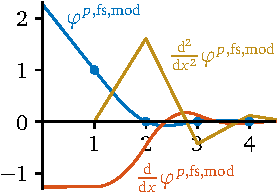
\includegraphics{modifiedFundamentalSpline_1}%
  }%
  \hfill%
  \subcaptionbox{%
    $p = 5$%
  }[48mm]{%
    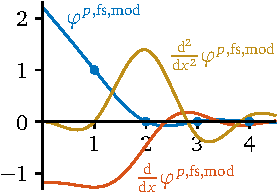
\includegraphics{modifiedFundamentalSpline_2}%
  }%
  \hfill%
  \subcaptionbox{%
    $p = 7$%
  }[48mm]{%
    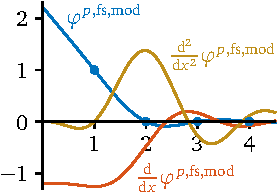
\includegraphics{modifiedFundamentalSpline_3}%
  }%
  \caption[%
    Modified fundamental spline and its derivatives%
  ]{%
    Modified fundamental spline $\parentfundspl[\modified]{p}$
    \emph{\textcolor{C0}{(blue)}} together with its
    first \emph{\textcolor{C1}{(red)}} and
    second \emph{\textcolor{C2}{(brown)}} derivatives
    and the function value interpolation conditions from
    \cref{eq:modifiedFundamentalSplineConditions}
    \emph{\textcolor{C0}{(blue dots)}.}
    For $p = 3$, the second derivative vanishes on
    $\clint{0, 1}$.
    For higher degrees $p > 3$, the second derivative is close to zero
    on this interval, vanishing at $x = 0$.%
  }%
  \label{fig:modifiedFundamentalSpline}%
\end{figure}

\vspace*{\fill}

The conditions stated in \eqref{eq:modifiedFundamentalSplineConditions}
are motivated by the case $p = 3$ of cubic fundamental splines.
The first relevant cardinal B-spline is the one with
index $k = 1 - \tfrac{p+1}{2}$ ($k = -1$ in the cubic case),
as the B-splines with indices $\le -\tfrac{p+1}{2}$ vanish on $\nonnegreal$.
The modified function $\parentfundspl[\modified]{p}$
should satisfy the fundamental property \eqref{eq:tiftDefinition}
at all positive integer points $k \in \nat$.
In contrast to the standard fundamental spline $\parentfundspl{p}$,
we do not enforce the fundamental property at $k = 0$,
as our aim is to obtain non-zero boundary values.
This leaves us exactly two degrees of freedom in the cubic case,
namely $k = -1$ and $k = 0$.
We use these to let $\parentfundspl[\modified]{p}$ extrapolate
linearly on $\clint{0, 1}$, as we did for uniform hierarchical
B-splines (see \cref{sec:313modification}).
\pagebreak
Therefore, in the cubic case, we set the second derivative
$\tderiv[2]{x}{\parentfundspl[\modified]{p}}$ to zero
at $x = 0$ and at $x = 1$.
This suffices since
$\tderiv[2]{x}{\parentfundspl[\modified]{p}}$ is piecewise
linear for $p = 3$.
For higher degrees $p > 3$,
we use the additional degrees of freedom (in total $\tfrac{p+1}{2}$)
to increase the multiplicity of the root of
$\tderiv[2]{x}{\parentfundspl[\modified]{p}}$ at $x = 0$.
This ensures that $\parentfundspl[\modified]{p}$ is
``as linear as possible'' near $x = 0$.
Note that we cannot maintain
$\tderiv[2]{x}{\parentfundspl[\modified]{p}} \equiv 0$
on $\clint{0, 1}$ for higher degrees $p > 3$,
since this would require $p - 1$ conditions,
and we only have $\tfrac{p+1}{2}$ degrees of freedom left,
after taking the fundamental conditions into account.



\subsection{Fundamental Not-A-Knot Splines}
\label{sec:445fundamentalNotAKnotSplines}

The hierarchical fundamental spline basis suffers from the same problem
as the uniform hierarchical B-spline basis.
As explained in \cref{sec:321approximation}, there is a mismatch
of dimensions of the nodal B-spline space $\nsbspl{l}{p}$ of level $l$
when compared with the spline space $\wholesplspace{l}{p}$ on the grid
$\{\gp{l,i} \mid i = 0, \dotsc, 2^l\}$ of level $l$.
This issue also affects the fundamental spline basis.

\paragraph{Definition of fundamental not-a-knot splines}

It is possible to combine the idea of fundamental splines
with the not-a-knot approach from \cref{sec:32notAKnot}.
We define hierarchical fundamental not-a-knot splines
$\bspl[\fs,\nak]{l',i'}{p}\colon \clint{0, 1} \to \real$ as
linear combinations of nodal not-a-knot B-splines of the same level,
where the coefficients are chosen such that the
fundamental property \eqref{eq:fundamentalProperty} is satisfied:
\begin{equation}
  \label{eq:fundamentalNotAKnotSplines}
  \bspl[\fs,\nak]{l',i'}{p}
  \ceq \sum_{i''=0}^{2^{l'}}
  \fundsplcoeff[l',i',\fs]{i''}{p} \bspl[\nak]{l',i''}{p}
  \quad\text{such that}\quad
  \falarge{i = 0, \dotsc, 2^{l'}}{
    \bspl[\fs,\nak]{l',i'}{p}(\gp{l',i}) = \kronecker{i}{i'}
  },
\end{equation}
where $l' \in \natz$, $i' = 0, \dotsc, 2^{l'}$, and
$\fundsplcoeff[l',i',\fs]{i''}{p} \in \real$.
This approach is similar to the \hftr in
\cref{sec:442constructingFundamentalBases},
see \cref{eq:hierarchicalFundamentalTransformation}.
We show the hierarchical fundamental not-a-knot spline basis
of cubic degree in \cref{fig:hierarchicalFundamentalNotAKnotSpline}.

The fundamental not-a-knot splines $\bspl[\fs,\nak]{l',i'}{p}$
of level $l' < \ceil{\log_2(p+1)}$ equal the Lagrange polynomials
$\lagrangepoly{l',i'}$ ($i' = 0, \dotsc, 2^{l'}$),
This is because the $i'$-th summand $\bspl[\nak]{l',i'}{p}$
of \eqref{eq:fundamentalNotAKnotSplines} equals $\lagrangepoly{l',i'}$ and
as $\lagrangepoly{l',i'}$ already fulfills the
fundamental interpolation conditions given in
\eqref{eq:fundamentalNotAKnotSplines}
(see \cref{eq:hierarchicalNotAKnotBSpline}),
we obtain $\fundsplcoeff[l',i',\fs]{i''}{p} = \kronecker{i'}{i''}$, i.e.,
$\bspl[\fs,\nak]{l',i'}{p} = \lagrangepoly{l',i'}$.

\begin{SCfigure}
  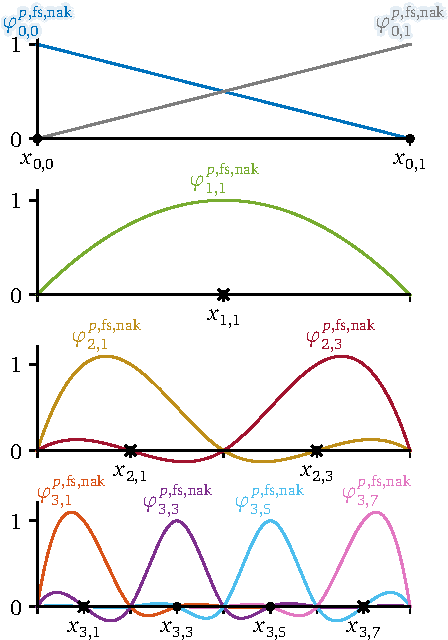
\includegraphics{hierarchicalBasis_16}%
  \caption[%
    Hierarchical fundamental not-a-knot splines%
  ]{%
    Hierarchical cubic fundamental not-a-knot splines
    $\bspl[\fs,\nak]{l',i'}{p}$
    ($l' \le l$, $i' \in \hiset{l'}$, $p = 3$),
    grid points $\gp{l',i'}$ \emph{(dots),} and
    removed knots \emph{(crosses)} up to level $l = 3$.%
  }%
  \label{fig:hierarchicalFundamentalNotAKnotSpline}%
\end{SCfigure}

\paragraph{Implementation}

We make two remarks with respect to the efficient implementation
of hierarchical fundamental not-a-knot splines.
First,
\cref{eq:fundamentalNotAKnotSplines} requires the solution of a system
of linear equations with dimension $2^{l'} + 1$,
which grows exponentially in the level~$l'$.
However, as the coefficients decay roughly in the same order
as the fundamental spline coefficients $\fundsplcoeff{k}{p}$ in
\cref{eq:fundamentalSplineCoefficientsDecay},
we can solve a truncated system of linear equations instead.

Second, the fundamental not-a-knot spline basis
$\bspl[\fs,\nak]{l',i'}{p}$ is not translation-invariant anymore.
This means that theoretically, we have to compute the
$\fundsplcoeff[l',i',\fs]{i''}{p}$ individually for each basis function
$\bspl[\fs,\nak]{l',i'}{p}$.
Nevertheless, when truncating the linear system for a fixed level $l'$,
almost all the inner basis functions $\bspl[\fs,\nak]{l',i'}{p}$
will be identical to hierarchical fundamental splines
$\bspl[\fs]{l',i'}{p}$, if the distance of the region with the removed knots
to the grid point $\gp{l',i'}$ is large enough
(if the removed knots are outside the truncated support of
$\bspl[\fs,\nak]{l',i'}{p}$).
For different levels $l'$, the fundamental not-a-knot splines
$\bspl[\fs,\nak]{l',i'}{p}$ are the same up to scaling
(if the level $l'$ is high enough).

Consequently, an efficient implementation only has to implement
$\bspl[\fs,\nak]{l',i'}{p}$ for some special cases for coarse levels.
The other basis functions can then be derived via an affine
parameter transformation.

\longsection{%
  \texorpdfstring{%
    Hierarchization on Spatially Adaptive Sparse Grids\\
    with the Unidirectional Principle%
  }{%
    Hierarchization on Spatially Adaptive Sparse Grids
    with the Unidirectional Principle%
  }%
}{%
  Hierarchization on Spatially Adaptive Sparse Grids
  with the Unidirectional Principle%
}{%
  Hierarchization with the Unidirectional Principle%
}
\label{sec:45spatAdaptiveUP}

\minitoc{90mm}{9}

\noindent
In this final section of the chapter,
we further decrease the computational complexity
for the application of the linear operator $\linop$
on spatially adaptive sparse grids
from quadratic to linear time with two algorithms based on the \up.



\subsection{%
  Iteratively Applying the Unidirectional Principle with Iterative Refinement%
}
\label{sec:451iterativeRefinement}

The first algorithm can be applied if two requirements are met:
\begin{itemize}
  \item
  The inverse $\linop^{-1}$ is known and can be efficiently applied.
  
  \item
  There is an operator $\linop'$
  that is ``sufficiently close'' to $\linop$ and can be efficiently applied.
\end{itemize}
For hierarchization with B-splines on sparse grids,
we choose $\linop$ to be the hierarchization
operator given in \cref{eq:hierarchizationSLE} and
$\linop'$ to be the \up directly applied on the
sparse grid.
Both of the assumptions are then satisfied,
as $\linop^{-1}$ is known
(interpolation matrix $\intpmat$ of basis function evaluations)
and $\linop^{-1}$ and $\linop'$ can be applied fast.
The \up $\linop'$ generally produces wrong
results for hierarchical B-splines due to missing coupling points.
However, especially for low B-spline degrees,
$\linop'$ does not deviate too much from the true operator $\linop$.
Below, we will specify a sufficient criterion for the ``closeness.''

\paragraph{Iterative refinement}

Under the two assumptions above, we can apply the procedure given in
\cref{alg:iterativeRefinement}.
The algorithm is equivalent to the well-known method of
\term{iterative refinement,} which has been developed to
stabilize the numerical solution of a linear system
influenced by rounding errors \cite{Higham02Accuracy}.
The operator $\linop'$ acts like a preconditioner,
which is why it is required to be close to $\linop$.
Note that the algorithm is similar to the repeated application
of the method of residual interpolation
(see \cref{sec:433residualInterpolation}) on the whole sparse grid.

\begin{algorithm}
  \begin{algorithmic}[1]
    \Function{$\vlinout = \texttt{iterativeRefinement}$}{%
      $\vlinin$, $\vlinout[(0)]$%
    }
      \State{$\*r^{(0)} \gets \vlinin - \linop^{-1}\vlinout[(0)]$}
      \Comment{initial residual}%
      \For{$m = 0, 1, 2, \dotsc$}
        \State{$\vlinout[(m+1)] \gets \vlinout[(m)] + \linop' \*r^{(m)}$}
        \Comment{update solution}%
        \State{$\*r^{(m+1)} \gets \*r^{(m)} - \linop^{-1} \linop' \*r^{(m)}$}
        \Comment{update residual}%
      \EndFor{}
      \vspace{-1mm}
      \State{$\vlinout \gets \text{last computed } \vlinout[(m)]$}
    \EndFunction{}
  \end{algorithmic}
  \caption[%
    Iterative refinement%
  ]{%
    Application of a tensor product operator $\linop$
    on spatially adaptive sparse grids with iterative refinement,
    where $\linop'$ is an approximation of $\linop$.
    Inputs are the vector $\vlinin = (\linin{\*l,\*i})_{(\*l,\*i) \in \liset}$
    of input data (function values $\fcnval{\*l,\*i}$ at the grid points) and
    an initial solution $\vlinout[(0)]$.
    The output is the vector
    $\vlinout = (\linout{\*l,\*i})_{(\*l,\*i) \in \liset}$
    of output data (hierarchical surpluses $\surplus{\*l,\*i}$).%
  }%
  \label{alg:iterativeRefinement}%
\end{algorithm}

The loop in \cref{alg:iterativeRefinement} has to be terminated
after some iterations.
The following simple lemma allows to use a stopping criterion based on the
size of the residual $\*r^{(m)}$ to the true solution,
which we denote with $\vlinout[\ast] \ceq \linop \vlinin$.

\begin{shortlemma}[equivalent convergence for iterative refinement]
  \label{lemma:iterativeRefinementEquivalent}
  In \cref{alg:iterativeRefinement}, we have
  $\vlinout[(m)] \to \vlinout[\ast] \iff \*r^{(m)} \to \*0$ for
  $m \to \infty$.
\end{shortlemma}

\vspace{-0.5em}

\begin{proof}
  It suffices to prove $\linop \*r^{(m)} = \vlinout[\ast] - \vlinout[(m)]$
  for $m \in \nat$ by induction.
  For $m = 0$, we have
  $\linop \*r^{(0)}
  = \linop \vlinin - \linop \linop^{-1} \vlinout[(0)]
  = \vlinout[\ast] - \vlinout[(0)]$.
  For $m \to m+1$, it holds
  $\linop \*r^{(m+1)}
  = \linop \*r^{(m)} - \linop \linop^{-1} \linop' \*r^{(m)}
  = (\vlinout[\ast] - \vlinout[(m)]) - \linop' \*r^{(m)}
  = \vlinout[\ast] - \vlinout[(m+1)]$.
\end{proof}

\vspace{0.5em}

\noindent
Next, we give a sufficient condition for the
convergence of \cref{alg:iterativeRefinement} to the true solution.

\vspace{0.5em}

\begin{proposition}[%
  sufficient condition for the convergence of
  {\hyperref[alg:iterativeRefinement]{Alg.\ \ref*{alg:iterativeRefinement}}}%
]
  \label{prop:iterativeRefinementSufficient}
  If we have $\limsup_{m \to \infty}
  \sqrt[m]{\norm{(\idop - \linop^{-1} \linop')^m}} < 1$
  with an arbitrary operator matrix norm $\norm{\cdot}$ and the
  identity operator $\idop$,
  then $\vlinout[(m)] \to \vlinout[\ast]$ for $m \to \infty$
  in \cref{alg:iterativeRefinement}
  for every initial solution $\vlinout[(0)]$.
\end{proposition}

\vspace{-0.5em}

\begin{proof}
  A short proof by induction shows that
  \begin{equation}
    \label{eq:proofPropIterativeRefinementSufficient}
    \vlinout[(m)]
    = \vlinout[(0)] + \linop'
    \sum_{m'=0}^{m-1} (\idop - \linop^{-1} \linop')^{m'} \*r^{(0)},
  \end{equation}
  where $(\idop - \linop^{-1} \linop')^{m'} \*r^{(0)} = \*r^{(m')}$.
  For $m \to \infty$ and with the assumption on
  $\norm{(\idop - \linop^{-1} \linop')^m}$,
  the sum converges to the Neumann series
  $\sum_{m'=0}^\infty (\idop - \linop^{-1} \linop')^{m'}
  = (\idop - (\idop - \linop^{-1} \linop'))^{-1} = (\linop')^{-1} \linop$
  (see, e.g., \cite{Werner11Funktionalanalysis}).
  In this case, we infer that the limit of $\vlinout[(m)]$ is given by
  \begin{equation}
    \vlinout[(0)] + \linop' (\linop')^{-1} \linop \*r^{(0)}
    = \vlinout[(0)] + \linop \vlinin - \linop \linop^{-1} \vlinout[(0)]
    = \linop \vlinin
    = \vlinout[\ast],
  \end{equation}
  as claimed.
\end{proof}

The sufficient condition given in \cref{prop:iterativeRefinementSufficient}
is quite strong, as it can be shown that $\limsup_{m \to \infty}
\sqrt[m]{\norm{(\idop - \linop^{-1} \linop')^m}} \le 1$ is necessary for
convergence.
Unfortunately, in the case of hierarchization with B-splines,
numerical experiments show that
this condition is only met for low dimensionalities $d$ and low
B-spline degrees $p$.
\Cref{alg:iterativeRefinement} generally diverges
for higher dimensionalities or higher degrees.



\subsection{Duality of the Unidirectional Principle}
\label{sec:452duality}

To motivate the second algorithm that we present in this section,
we study why we cannot directly apply the \up
(as introduced in \cref{alg:unidirectionalPrinciple})
on spatially adaptive sparse grids.
As before, we denote with $\liset$ the level-index set of
the spatially adaptive sparse grid (see \cref{sec:41problem}).

The \up\punctfix{,} as stated in
\cref{alg:unidirectionalPrinciple} for full grids,
subsequently applies one-dimensional operators
$\upopuv{t_j}{\lisetpole}\colon \real^{\setsize{\lisetpole}} \to
\real^{\setsize{\lisetpole}}$
on the poles $\lisetpole$ of the sparse grid at hand,
iterating over a permutation $t_1, \dotsc, t_d$
of the dimensions $1, \dotsc, d$.
We recall the pole equivalence relation $\samepole{t_j}$
from \cref{eq:poleEquivalenceRelation}:
Two points $\*k', \*k'' \in \liset$ are $\samepole{t_j}$-equivalent,
if $\*k'$ is contained in the pole through $\*k''$
with respect to the $t_j$-th dimension, i.e.,
\begin{equation}
  \*k' \samepole{t_j} \*k'' \iff \*k'_{-t_j} = \*k''_{-t_j},\quad
  \*k', \*k'' \in \liset.
\end{equation}

\paragraph{Operators for the unidirectional principle}

The combined application of all one-di\-men\-sional operators
$\upopuv{t_j}{\lisetpole}$
($\lisetpole \in \eqclasses{\liset}{\samepole{t_j}}$)
of the $j$-th iteration of \cref{alg:unidirectionalPrinciple}
is equivalent to a single application of the following operator
$\upop{t_j}\colon \real^{\setsize{\liset}} \to \real^{\setsize{\liset}}$:
\begin{equation}
  \label{eq:upopEntries}
  (\upop{t_j})_{\*k'',\*k'}
  \ceq
  \begin{cases}
    (\upopuv{t_j}{\lisetpole})_{k''_{t_j},k'_{t_j}},&
    \ex{\lisetpole \in \eqclasses{\liset}{\samepole{t_j}}}{
      \*k', \*k'' \in \lisetpole
    },\\
    0,&\*k' \not\samepole{t_j} \*k'',
  \end{cases}
\end{equation}
where $(\upop{t_j})_{\*k'',\*k'}$ denotes the entry of row $\*k''$
and column $\*k'$ of the matrix corresponding to $\upop{t_j}$
(similar for $(\upopuv{t_j}{\lisetpole})_{k''_{t_j},k'_{t_j}}$).
The reason for this equivalence is that
the poles $\lisetpole$ are pairwise disjoint equivalence classes.
Consequently, every point $\*k$ is only acted upon by a single
one-dimensional operator $\upopuv{t_j}{\lisetpole}$,
namely the one with $\lisetpole = \eqclass{\*k}{\samepole{t_j}}$.
This leads to the block-diagonal structure
of $\upop{t_j}$ given in \eqref{eq:upopEntries},
if the rows of the matrix of $\upop{t_j}$
are grouped by poles $\lisetpole$ and the columns are arranged accordingly.

\paragraph{Correctness and duality of the unidirectional principle}

For the remaining considerations, we assume that
the operators $\linop$ and $\upopuv{t_j}{\lisetpole}$ are invertible.
In this case, $\upop{t_j}$ is also invertible and
$\upopinv{t_j}$ is given by the block-diagonal matrix composed of
the inverses of the blocks $\upopuv{t_j}{\lisetpole}$ of $\upop{t_j}$.
This is satisfied by dehierarchization operators $\intpmat$ due to the
linear independence of the hierarchical basis functions.

We are now able to describe the whole \up of
\cref{alg:unidirectionalPrinciple} as the operator
$\upop{t_1,\dotsc,t_d}\colon \real^{\setsize{\liset}} \to
\real^{\setsize{\liset}}$ given by
\begin{equation}
  \label{eq:upopProduct}
  \upop{t_1,\dotsc,t_d}
  \ceq \upop{t_d} \dotsm \upop{t_1}.
\end{equation}
The right-most operator is $\upop{t_1}$, since it is applied first.
We say that the \up is \term{correct} for $\linop$ and
$(t_1, \dotsc, t_d)$, if
\begin{equation}
  \upop{t_1,\dotsc,t_d}
  \overset{?}{=} \linop.
\end{equation}
This relation is not satisfied in general,
especially for B-spline hierarchization with the operator
$\linop = \intpmatinv$.
However, for operators like these, whose inverse
$\linopinv = \intpmat$ can be described and applied much easier,
we can make use of the so-called \term{duality of the \up:}

\begin{lemma}[duality of the unidirectional principle]
  \label{lemma:dualityUnidirectionalPrinciple}
  Let the operators $\linop$ and $\upopuv{t_j}{\lisetpole}$ be invertible
  for all poles $\lisetpole$ in $\liset$.
  Then the \up is correct for $\linop$ and $(t_1, \dotsc, t_d)$
  if and only if the \up is correct for $\linopinv$ and $(t_d, \dotsc, t_1)$.
\end{lemma}

\begin{proof}
  The correctness of the \up for $\linop$ and $(t_1, \dotsc, t_d)$
  is by definition equivalent to
  \begin{equation}
    \upop{t_d} \dotsm \upop{t_1} = \linop.
  \end{equation}
  By inverting both sides, we obtain the definition of the
  correctness of the \up for $\linopinv$ and $(t_d, \dotsc, t_1)$.
\end{proof}

This duality means that in order to establish the correctness of $\linop$
for some arbitrary permutation $(t_1, \dotsc, t_d)$ of $1, \dotsc, d$,
it suffices to establish the \up's correctness for the
inverse operator $\linopinv$ and the reverse permutation $(t_d, \dotsc, t_1)$.
This is especially of interest for our main application,
the hierarchization operator $\linop = \intpmatinv$ for B-splines.



\subsection{Chains and Equivalent Correctness Conditions}
\label{sec:453chains}

We first define the notion of a chain between two grid points
$\*k'$ and $\*k''$.

\begin{definition}[chain]
  \label{def:chain}
  Let $\*k', \*k'' \in \liset$ and
  $(t_1, \dotsc, t_j)$ be a permutation of $j$ of the
  dimensions $1, \dotsc, d$.
  We define the \term{chain} from $\*k'$ to $\*k''$ with respect to
  $(t_1, \dotsc, t_j)$ as the sequence
  $(\chain{0}, \dotsc, \chain{j})$, where
  \begin{equation}
    \chain{j'}_{T_{j'}}
    \ceq \*k''_{T_{j'}},\quad
    \chain{j'}_{-T_{j'}}
    \ceq \*k'_{-T_{j'}},\quad
    T_{j'}
    \ceq (t_1, \dotsc, t_{j'}),\quad
    j' = 0, \dotsc, j,
    \hspace*{-10mm}
  \end{equation}
  if $\chain{j} = \*k''$ and
  $\chain{j'} \in \liset$ for all $j' = 0, \dotsc, j$.
\end{definition}

This definition is equivalent to
$\chain{j'-1} \samepole{t_{j'}} \chain{j'}$ for $j' = 1, \dotsc, j$.
\Cref{fig:chainDefinition} shows examples of chains in
two and three dimensions.
As it is shown in \cref{fig:chainDefinition2},
the order $(t_1, \dotsc, t_j)$ of the dimensions is important
for whether the grid contains the chain from $\*k'$ to $\*k''$.
The grid must contain all intermediate points, otherwise
it is not a chain.

\begin{figure}
  \subcaptionbox{%
    $d = 2$, $(t_1, t_2) = (2, 1)$%
  }[47mm]{%
    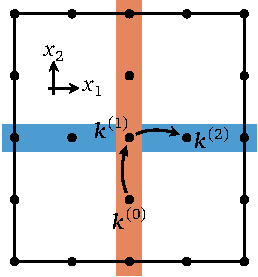
\includegraphics{chainDefinition_1}%
  }%
  \hfill%
  \subcaptionbox{%
    $d = 2$, $(t_1, t_2) = (1, 2)$%
    \label{fig:chainDefinition2}%
  }[47mm]{%
    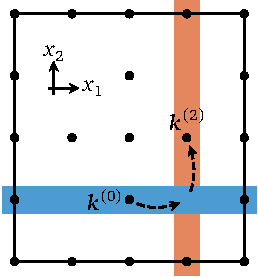
\includegraphics{chainDefinition_2}%
  }%
  \hfill%
  \subcaptionbox{%
    $d = 3$, $(t_1, t_2, t_3) = (2, 3, 1)$%
  }[50mm]{%
    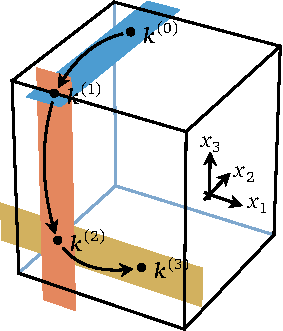
\includegraphics{chainDefinition_3}%
  }%
  \caption[%
    Examples for the definition of chains%
  ]{%
    Examples for chains in two and three dimensions.
    \emph{Left:} A chain from $\chain{0}$ to $\chain{2}$
    with respect to $(t_1, t_2) = (2, 1)$ in a two-dimensional sparse grid.
    \emph{Center:}
    With respect to the reverse permutation
    $(t_1, t_2) = (1, 2)$ of the dimensions,
    there is no chain from $\chain{0}$ to $\chain{2}$,
    because the corresponding chain point $\chain{1}$ is missing in the grid.
    \emph{Right:} A chain in three dimensions.%
  }%
  \label{fig:chainDefinition}%
\end{figure}

We now show two lemmas.
First, we prove that $(\upop{t_1,\dotsc,t_j})_{\*k'',\*k'} \not= 0$
is sufficient for the existence of a chain from $\*k'$ to $\*k''$:

\begin{restatable}[sufficient condition for chain existence]{%
  lemma%
}{%
  lemmaChainExistenceSufficient%
}
  \label{lemma:chainExistenceSufficient}
  If $(\upop{t_1,\dotsc,t_j})_{\*k'',\*k'} \not= 0$
  for some $j = 0, \dotsc, d$,
  then the grid $\liset$ contains the chain from $\*k'$ to $\*k''$
  with respect to $(t_1, \dotsc, t_j)$.
\end{restatable}

\vspace{-0.5em}

\begin{proof}
  See \cref{sec:a134proofCorrectnessUnidirectionalPrincipleSASG}.
\end{proof}

\vspace{0.5em}

Second, we show that the equality of
$(\upop{t_1,\dotsc,t_j})_{\chain{j},\*k'}$ and the product of
the one-dimensional operators is necessary for the
existence of a chain from $\*k'$ to $\*k''$:

\begin{restatable}[necessary condition for chain existence]{%
  lemma%
}{%
  lemmaChainExistenceNecessary%
}
  \label{lemma:chainExistenceNecessary}
  If the grid $\liset$ contains the chain $(\chain{0}, \dotsc, \chain{j})$
  from $\*k'$ to $\*k''$ with respect to $(t_1, \dotsc, t_j)$
  for some $j = 0, \dotsc, d$, then
  \begin{equation}
    \label{eq:lemmaChainExistenceNecessary}
    (\upop{t_1,\dotsc,t_j})_{\chain{j},\*k'}
    = (\upopuv{t_1}{\eqclass{\chain{1}}{\samepole{t_1}}})_{k''_{t_1},k'_{t_1}}
    \dotsm
    (\upopuv{t_j}{\eqclass{\chain{j}}{\samepole{t_j}}})_{k''_{t_j},k'_{t_j}}.
  \end{equation}
\end{restatable}

\vspace{-0.5em}

\begin{proof}
  See \cref{sec:a134proofCorrectnessUnidirectionalPrincipleSASG}.
\end{proof}

\vspace{0.5em}

These two lemmas can be used to prove the following characterization
of the correctness of the \up\punctfix{.}
Here, we need an additional assumption on the structure of the
operator $\linop$, which we call \term{tensor product structure:}

\begin{restatable}[characterization of the correctness of the UP]{%
  proposition%
}{%
  propCorrectnessUPCharacterization%
}
  \label{prop:correctnessUPCharacterization}
  Let $\linop$ have tensor product structure:
  For all $\*k', \*k'' \in \liset$ with the chain
  $(\chain{0}, \dotsc, \chain{d})$ from $\*k'$ to $\*k''$
  with respect to $(t_1, \dotsc, t_d)$,
  we assume that
  \begin{equation}
    \label{eq:tensorProductOperator}
    (\linop)_{\*k'',\*k'}
    = \prod_{j=1}^d
    (\upopuv{t_j}{\eqclass{\chain{j}}{\samepole{t_j}}})_{k''_{t_j},k'_{t_j}}.
  \end{equation}
  Then the \up is correct for $\linop$ and $(t_1, \dotsc, t_d)$
  if and only if the grid $\liset$ contains the chain from $\*k'$ to $\*k''$
  with respect to $(t_1, \dotsc, t_d)$ for all $\*k', \*k'' \in \liset$
  for which $(\linop)_{\*k'',\*k'} \not= 0$.
\end{restatable}

\vspace{-0.5em}

\begin{proof}
  See \cref{sec:a134proofCorrectnessUnidirectionalPrincipleSASG}.
\end{proof}

\vspace{0.5em}

When applied to the hierarchization operator,
the combination of \cref{prop:correctnessUPCharacterization} with
\thmref{lemma:dualityUnidirectionalPrinciple} can be summarized in
the following corollary:

\begin{corollary}[%
  equivalent statements for correctness of UP for hierarchization%
]
  \label{cor:equivalentCorrectnessUPHierarchization}
  The following statements are equivalent:
  \begin{itemize}
    \item
    The \up is correct for $\intpmatinv$ and $(t_1, \dotsc, t_d)$.
    
    \item
    The \up is correct for $\intpmat$ and $(t_d, \dotsc, t_1)$.
    
    \item
    The grid $\liset$ contains the chain from $\*k'$ to $\*k''$
    with respect to $(t_d, \dotsc, t_1)$ for all $\*k', \*k'' \in \liset$
    for which $\basis{\*k'}(\gp{\*k''}) \not= 0$.
  \end{itemize}
\end{corollary}

\begin{proof}
  The corollary is a direct consequence of
  \cref{lemma:dualityUnidirectionalPrinciple} and
  \cref{prop:correctnessUPCharacterization},
  applied to the dehierarchization operator $\linop = \intpmat$.
  
  The assumption of \cref{lemma:dualityUnidirectionalPrinciple}
  is satisfied:
  The operators $\upopuv{t_j}{\lisetpole}$ are invertible
  for all poles $\lisetpole$ in $\liset$
  due to the uniqueness of univariate interpolants
  (linear independence of the basis functions).
  Similarly, $\linop$ is invertible
  due to the uniqueness of multivariate interpolants.
  In addition, the assumption of \cref{prop:correctnessUPCharacterization}
  is satisfied, since
  \begin{equation}
    (\linop)_{\*k'',\*k'}
    = (\intpmat)_{\*k'',\*k'}
    = \prod_{j=1}^d \basis{k'_{t_j}}(\gp{k''_{t_j}})
    = \prod_{j=1}^d
    (\upopuv{t_j}{\eqclass{\chain{j}}{\samepole{t_j}}})_{k''_{t_j},k'_{t_j}}
  \end{equation}
  due to the tensor product basis functions.
\end{proof}

\paragraph{Inserting chain points}

This means that we can establish the correctness of the \up
for the hierarchization operator $\linop = \intpmatinv$,
if we insert all missing chain points that are specified by
\cref{prop:correctnessUPCharacterization} into the grid.

We take the case $p = 1$ of piecewise linear
standard B-splines $\bspl{\*l,\*i}{1}$ as an example.
We assume that we iteratively generated a spatially adaptive sparse grid
such that all grid points are reachable from the corners of $\clint{\*0, \*1}$
in the sense of \cref{eq:bfsAssumption2}.
If we want to ensure the correctness of the \up for all possible permutations
$(t_1, \dotsc, t_d)$ of the dimensions $(1, \dotsc, d)$,
then the existence of the necessary chains in
\cref{cor:equivalentCorrectnessUPHierarchization} is equivalent to the
requirement that the grid should contain
the hierarchical ancestors of every grid point in every direction:
\begin{subequations}
  \begin{alignat}{4}
    \fafa{(\*l',\*i') \in \liset}{\{t = 1, \dotsc, d \mid l'_t > 1\}}{
      (\*l,\*i) \in \liset
    },\quad
    &&&\*l \ceq \*l' - \stdbasis{t},\quad
    &&i_t \ceq 2 \floor{\tfrac{i'_t}{4}} + 1,\quad
    &&\*i_{-t} = \*i'_{-t},\\
    \fafa{(\*l',\*i') \in \liset}{\{t = 1, \dotsc, d \mid l'_t = 1\}}{
      (\*l,\*i) \in \liset
    },\quad
    &&&\*l \ceq \*l' - \stdbasis{t},\quad
    &&i_t \ceq 0,\quad
    &&\*i_{-t} = \*i'_{-t},
  \end{alignat}
\end{subequations}
where $\stdbasis{t}$ is the $t$-th standard basis vector.
This is a standard assumption on spatially adaptive sparse grids with
piecewise linear basis functions \cite{Pflueger10Spatially}.
However, we only have to satisfy the conditions of
\cref{cor:equivalentCorrectnessUPHierarchization} for a single permutation
$(t_1, \dotsc, t_d)$ of the dimensions
in order to hierarchize with the \up\punctfix{.}
\Cref{fig:chainInsertionBSpline} shows the necessary ancestor chain points
(colored points in \cref{fig:chainInsertionBSpline2})
for an example of a two-dimensional spatially adaptive sparse grid
(\cref{fig:chainInsertionBSpline1}).

\begin{figure}
  \subcaptionbox{%
    Original grid ($N = 85$)%
    \label{fig:chainInsertionBSpline1}%
  }[48mm]{%
    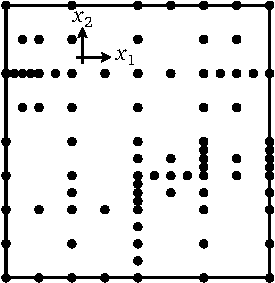
\includegraphics{chainInsertion_1}%
  }%
  \hfill%
  \subcaptionbox{%
    Chain points for $p = 1$\\
    \rlap{\hspace*{10.5mm}($N = 121$)}%
    \label{fig:chainInsertionBSpline2}%
  }[48mm]{%
    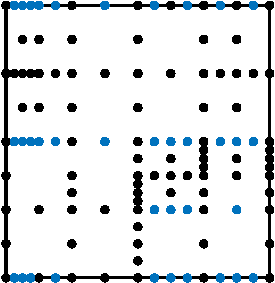
\includegraphics{chainInsertion_2}%
  }%
  \hfill%
  \subcaptionbox{%
    Chain points for $p = 3$\\
    \rlap{\hspace*{10.5mm}($N = 289 = 17 \times 17$)}%
    \label{fig:chainInsertionBSpline3}%
  }[48mm]{%
    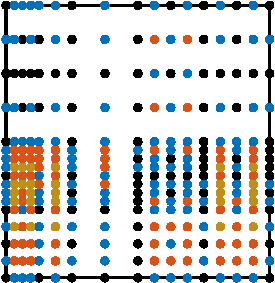
\includegraphics{chainInsertion_3}%
  }%
  \caption[%
    Chain points for hierarchical B-splines on a sparse grid%
  ]{%
    Necessary chain points for the correctness of the unidirectional principle
    with respect to $(t_1, t_2) = (1, 2)$
    for hierarchical B-splines $\bspl{l,i}{p}$ on a
    two-dimensional spatially adaptive sparse grid.
    The colors indicate the recursion depth in which the
    chain points have been inserted.
    Black points are contained in the original grid
    (``zero-order points'').
    \textcolor{C0}{Blue points} are part of chains
    between original grid points (``first-order chain points'').
    \textcolor{C1}{Red points} are second-order chain points,
    i.e., they are part of chains
    from $\*k'$ to $\*k''$ where $\*k'$ and $\*k''$ are
    original grid points or first-order chain points
    and at least one of them is a first-order chain point.
    Analogously,
    \textcolor{C2}{brown points} are third-order chain points.
    $N$ is the number of points in the final grid.%
  }%
  \label{fig:chainInsertionBSpline}%
\end{figure}

Unfortunately, we have to insert these points recursively,
e.g., the inserted points may generate new chains,
for which other missing points have to be inserted and so on
(``higher-order chain points'' in \cref{fig:chainInsertionBSpline}).
Therefore, the number of points to be inserted may be large.
The worst case is that the final grid is a full grid, i.e.,
the Cartesian product of the union of the poles in the different dimensions:
\begin{equation}
  \paren*{\bigcup_{\*k \in \liset} \eqclass{\*k}{\samepole{1}}}
  \times \dotsb \times
  \paren*{\bigcup_{\*k \in \liset} \eqclass{\*k}{\samepole{d}}},
\end{equation}
i.e., we fully lose the advantage of sparse grids,
whose purpose is to ease the curse of dimensionality.
For the standard hierarchical B-spline basis $\bspl{l,i}{p}$,
this worst case often occurs as there are many non-zero entries
in the corresponding interpolation matrices $\intpmat$
(see \cref{sec:41problem} and \cref{fig:chainInsertionBSpline3}).



\subsection{Hierarchical Weakly Fundamental Splines}
\label{sec:454wfs}

\paragraph{Motivation}

In order to reduce the number of chain points to be inserted,
we have to use other spline bases such that
the resulting interpolation matrices $\intpmat$ have more zero entries.
The hierarchical fundamental splines
as introduced in \cref{sec:443fundamentalSplines} are one possibility.
However, they are globally supported, which implies a number
of disadvantages concerning the algorithms and the implementations.
The most significant disadvantage is that although
we can use \bfs for the univariate hierarchization operators,
the time complexity for the univariate hierarchization is still quadratic.
We search for a locally supported spline basis for which
the univariate hierarchization can be done in linear time.

To meet these goals, we have to relax the fundamental property
to a weaker version, which results in the so-called
\term{weakly fundamental property.}
A univariate hierarchical basis
$\wfundbasis{l',i'}\colon \clint{0, 1} \to \real$
is called \term{weakly fundamental,} if
\begin{equation}
  \label{eq:weaklyFundamentalProperty}
  \wfundbasis{l',i'}(\gp{l,i}) = 0,\quad
  l < l',\;\;
  i \in \hiset{l}.
\end{equation}
This is exactly the first condition \eqref{eq:fundamentalProperty1}
of the fundamental property \eqref{eq:fundamentalProperty}.
We drop the requirement that the basis functions
should vanish at the other grid points of the same level.
The relation \eqref{eq:fundamentalPropertyImplicationMV} from the
fundamental case becomes
\begin{equation}
  \label{eq:weaklyFundamentalPropertyImplicationMV}
  \wfundbasis{\*l',\*i'}(\gp{\*l,\*i})
  \not= 0
  \implies
  \*l' \le \*l,
\end{equation}
i.e., every basis function $\wfundbasis{\*l',\*i'}$
can only be non-zero at grid points $\gp{\*l,\*i}$ with
higher or equal level $\*l$.

\paragraph{Definition of hierarchical weakly fundamental splines}

We construct the \term{weakly fundamental spline parent function}
$\parentwfundspl{p}\colon \real \to \real$
by forming a linear combination of as few neighboring
uniform B-splines as possible such that $\parentwfundspl{p}$
satisfies the weakly fundamental property
\eqref{eq:weaklyFundamentalProperty}:
\begin{subequations}
  \begin{gather}
    \label{eq:weaklyFundamentalSplineParent}
    \parentwfundspl{p}(x)
    \ceq \largesum[(p-1)/2]{k=-(p-1)/2}
    \wfundsplcoeff{k}{p} \parentbspl{p}(x - k)
    \quad\text{such that}\\
    \wfundsplcoeff{0}{p} = 1,\quad
    \parentwfundspl{p}(k') = 0,\;\;
    k' = -p + 2,\; -p + 4,\; \dotsc,\; p - 2.
  \end{gather}
\end{subequations}
\usenotation{zzzzwfs}
\term{Hierarchical weakly fundamental splines}
$\bspl[\wfs]{l,i}{p}\colon \clint{0, 1} \to \real$
are now defined canonically via an affine parameter transformation:
\begin{equation}
  \bspl[\wfs]{l,i}{p}(x)
  \ceq \parentwfundspl{p}(\tfrac{x}{\ms{l}} - i),\quad
  l \ge 1.
\end{equation}
For $l = 0$, we define $\bspl[\wfs]{l,i}{p}$ to be the
linear Lagrange polynomial of level zero:%
\footnote{%
  This will simplify the description of the
  Hermite hierarchization algorithm in \cref{sec:455hermiteHierarchization}.%
}
\begin{equation}
  \bspl[\wfs]{0,i}{p}
  \ceq \lagrangepoly{0,i},\quad
  i = 0, 1.
\end{equation}
The hierarchical weakly fundamental spline basis is shown in
\cref{fig:hierarchicalWeaklyFundamentalSpline}.
Note that these basis functions are translation-invariant by construction
(starting with level $l \ge 1$).
As the weakly fundamental parent spline $\parentwfundspl{p}$
vanishes at all odd integers and as the
support of $\bspl[\wfs]{l,i}{p}$ is local
($\supp \bspl[\wfs]{l,i}{p}
= \clint{\gp{l,i-p}, \gp{l,i+p}} \cap \clint{0, 1}$),
this implies that the weakly fundamental property
\eqref{eq:weaklyFundamentalProperty} is fulfilled.

\begin{SCfigure}
  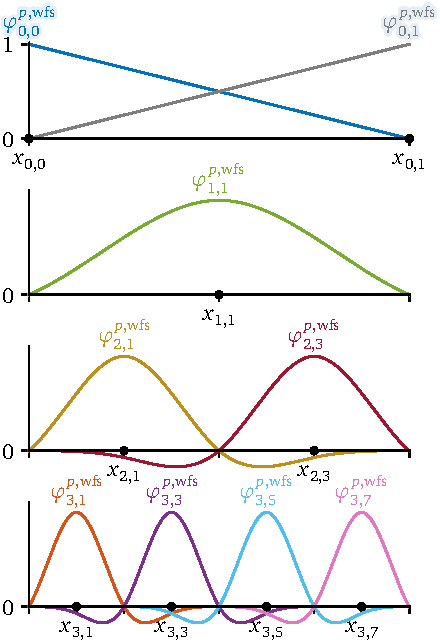
\includegraphics{hierarchicalBasis_17}%
  \caption[%
    Hierarchical weakly fundamental splines%
  ]{%
    Hierarchical cubic weakly
    \vspace{-0.1em}%
    fundamental splines
    $\bspl[\wfs]{l',i'}{p}$
    ($l' \le l$, $i' \in \hiset{l'}$, $p = 3$) and
    grid points $\gp{l',i'}$ \emph{(dots)} up to level $l = 3$.%
  }%
  \label{fig:hierarchicalWeaklyFundamentalSpline}%
\end{SCfigure}

\paragraph{Chain points for weakly fundamental splines}

The first advantage of the
weakly fundamental spline basis $\bspl[\wfs]{l,i}{p}$
over standard uniform B-splines $\bspl{l,i}{p}$ is that
the condition $\basis{\*k'}(\gp{\*k''}) \not= 0$ in
\cref{cor:equivalentCorrectnessUPHierarchization} is
satisfied for much fewer $\*k', \*k''$.
Consequently, fewer chain grid points have to be inserted to
ensure the correctness of the \up for hierarchization.
\Cref{fig:chainInsertionWeaklyFundamentalSpline} shows the inserted points
for the same grid as in \cref{fig:chainInsertionBSpline}.

\begin{SCfigure}
  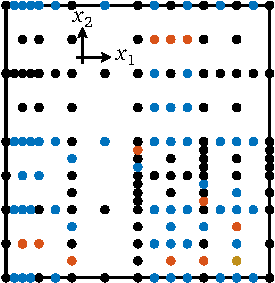
\includegraphics{chainInsertion_4}%
  \caption[%
    Chain points for hierarchical weakly fundamental splines on a
    sparse grid%
  ]{%
    Necessary chain points for the correctness of the unidirectional principle
    with respect to $(t_1, t_2) = (1, 2)$
    for hierarchical cubic weakly fundamental splines
    $\bspl[\wfs]{l,i}{p}$ ($p = 3$)
    on the same two-dimensional spatially adaptive sparse grid
    as in \cref{fig:chainInsertionBSpline1}.
    The colors indicate the recursion depth in which the
    chain points have been inserted
    (see caption of \cref{fig:chainInsertionBSpline}).
    The number of points in the final grid is $N = 157$.%
  }%
  \label{fig:chainInsertionWeaklyFundamentalSpline}%
\end{SCfigure}

In the special case of regular sparse grids $\regsgset{n}{d}$,
we do not have to insert any grid points for the correctness of the
\up\punctfix{.}
We can verify this statement with
\thmref{cor:equivalentCorrectnessUPHierarchization}:
Let $(\*l',\*i')$ and $(\*l'',\*i'')$ with
$\normone{\*l'}, \normone{\*l''} \le n$ and
$\*i' \in \hiset{\*l'}$, $\*i'' \in \hiset{\*l''}$,
such that $\bspl[\wfs]{\*l',\*i'}{p}(\gp{\*l'',\*i''}) \not= 0$.
Furthermore, let $(\chain[\*l]{0}, \chain[\*i]{0}), \dotsc,
(\chain[\*l]{d}, \chain[\*i]{d})$ be the chain
from $\*k'$ to $\*k''$ with respect to $t_1, \dotsc, t_d$.
Note that $\chain[\*l]{j} \le \vecmax\{\*l', \*l''\}$ due to the
definition of chain points (\cref{def:chain}).
Therefore, we have for $j = 0, \dotsc, d$
by \eqref{eq:weaklyFundamentalPropertyImplicationMV}:
\begin{equation}
\*l' \le \*l''
\implies
\chain[\*l]{j} \le \vecmax\{\*l', \*l''\} \le \*l''
\implies
\normone{\chain[\*l]{j}} \le \normone{\*l''} \le n.
\end{equation}
Hence, $\regsgset{n}{d}$ contains the grid points corresponding to
$(\chain[\*l]{j}, \chain[\*i]{j})$ for all $j = 0, \dotsc, d$.
Consequently, the conditions of
\cref{cor:equivalentCorrectnessUPHierarchization} are satisfied without
inserting any additional chain points.
This statement is even valid for arbitrary
dimensionally adaptive sparse grids.



\subsection{Hermite Hierarchization}
\label{sec:455hermiteHierarchization}

\paragraph{Hermite interpolation}

The second advantage of the weakly fundamental spline basis
is that due to the reduced coupling,
the univariate hierarchization operators can be applied easier
than for standard uniform B-splines.
This results in the formulation of the so-called
\term{Hermite hierarchization} algorithm.
We first recall higher-order Hermite interpolation:

\begin{lemma}[higher-order Hermite interpolation]
  \label{lemma:hermiteInterpolation}
  Let $p \in \nat$ be odd and $a, b \in \real$ with $a < b$.
  Furthermore, let
  $\deriv[q]{x}{\objfun}(a) \in \real$ and
  $\deriv[q]{x}{\objfun}(b) \in \real$ be given data
  for $q = 0, \dotsc, \frac{p-1}{2}$.
  Then there is a unique polynomial $\spl \in \polyspace{p}$ such that
  \begin{equation}
    \deriv[q]{x}{\objfun}(a)
    = \deriv[q]{x}{\spl}(a),\quad
    \deriv[q]{x}{\objfun}(b)
    = \deriv[q]{x}{\spl}(b),\quad
    q = 0, \dotsc, \frac{p-1}{2}.
    \hspace*{-10mm}
  \end{equation}
\end{lemma}

\begin{proof}
  See \cite{Freund07Stoer}.
\end{proof}

\paragraph{Hermite hierarchization algorithm}

The interpolating polynomial $\spl$ and its derivatives can be
efficiently evaluated using Hermite basis functions
(generalized Lagrange polynomials \cite{Freund07Stoer}).
With Hermite interpolation, we formulate
\cref{alg:hermiteHierarchization}
for the hierarchization with hierarchical weakly fundamental splines.
While we formulate \cref{alg:hermiteHierarchization}
only for regular univariate grids and weakly fundamental splines,
a slightly reformulated version of the algorithm
also correctly operates on spatially adaptive univariate grids
(with the assumption that the grids contain the parents of their grid points)
and other weakly fundamental bases that are
piecewise polynomials of degree $\le p$.

\begin{algorithm}
  \begin{algorithmic}[1]
    \Function{$\vlinout = \texttt{hermiteHierarchization1D}$}{%
      $\vlinin$, $n$%
    }
      \For{$i = 0, 1$}
      \Comment{set values for level $0$}%
        \State{%
          $\linout{0,i} \gets \fcnval{0,i}$%
        }
        \label{line:algHermiteHierarchization1}
        \State{%
          $\deriv[q]{x}{\fgintp{0}}(\gp{0,i})
          \gets \kronecker{q}{0} \cdot \fcnval{0,i} +
          \kronecker{q}{1} \cdot (\fcnval{0,1} - \fcnval{0,0})$
          for all $q = 0, \dotsc, \frac{p-1}{2}$%
        }
        \label{line:algHermiteHierarchization3}
      \EndFor{}
      \For{$l = 1, \dotsc, n$}
        \For{$i \in \hiset{l}$}
          \State{%
            $\fgintp{l-1}(\gp{l,i}) \gets \text{Hermite interpolation of}$
            $\deriv[q]{x}{\fgintp{l-1}}(\gp{l,i\pm1})$
            ($q = 0, \dotsc, \frac{p-1}{2}$)%
          }
          \label{line:algHermiteHierarchization4}
          \State{%
            $r^{(l)}(\gp{l,i})
            \gets \fcnval{l,i} - \fgintp{l-1}(\gp{l,i})$%
          }
          \label{line:algHermiteHierarchization5}
          \Comment{residual to be interpolated}%
        \EndFor{}
        \State{%
          Let $r^{(l)}_l$ be of the form
          $\sum_{i' \in \hiset{l}} \linout{l,i'} \bspl[\wfs]{l,i'}{p}$%
        }
        \Comment{contribution of level $l$}%
        \label{line:algHermiteHierarchization6}
        \State{%
          Choose $(\linout{l,i'})_{i' \in \hiset{l}}$ such that
          $r^{(l)}_l(\gp{l,i}) = r^{(l)}(\gp{l,i})$ for all $i \in \hiset{l}$%
        }
        \label{line:algHermiteHierarchization7}
        \For{$i = 0, \dotsc, 2^l$}
        \Comment{for all points (current level and ancestors)}%
          \For{$q = 0, \dotsc, \frac{p-1}{2}$}
            \State{%
              $\deriv[q]{x}{\fgintp{l}}(\gp{l,i})
              \gets \deriv[q]{x}{\fgintp{l-1}}(\gp{l,i}) +
              \deriv[q]{x}{r^{(l)}_l}(\gp{l,i})$%
            }
            \Comment{update values}%
            \label{line:algHermiteHierarchization8}
          \EndFor{}
        \EndFor{}
      \EndFor{}
    \EndFunction{}
  \end{algorithmic}
  \caption[%
    Hermite hierarchization%
  ]{%
    Hermite hierarchization on one-dimensional regular grids.
    Inputs are
    the vector $\vlinin = (\linin{l,i})_{(l,i) \in \liset}$
    of input data (function values $\fcnval{l,i}$ at the grid points) and
    the level $n$ of the regular grid,
    where $\liset = \{(l, i) \mid l = 0, \dotsc, n,\; i \in \hiset{l}\}$.
    The output is the vector
    $\vlinout = (\linout{l,i})_{(l,i) \in \liset}$
    of output data (hierarchical surpluses $\surplus{l,i}$).%
  }%
  \label{alg:hermiteHierarchization}%
\end{algorithm}

\vspace*{\fill}

The idea of \cref{alg:hermiteHierarchization},
which is also illustrated in \cref{fig:hermiteHierarchization},
is to hierarchize the function value data level by level,
which is only possible because of the weakly fundamental property
\eqref{eq:weaklyFundamentalProperty}.
For each level $l$, we calculate surpluses
$\surplus{l,i} = \linout{l,i}$, while keeping track of
the values and derivatives
$\deriv[q]{x}{\fgintp{l}}(\gp{l,i})$ of the
``current'' interpolant $\fgintp{l}$ (up to level $l$).
Hermite interpolation is used to determine the ``delta''
to the interpolant of the next level.
Note that in \cref{line:algHermiteHierarchization8},
we have to evaluate the derivatives of
$\deriv[q]{x}{\fgintp{l-1}}(\gp{l,i})$ of the Hermite interpolant
determined in \cref{line:algHermiteHierarchization4}.
This is not an issue since in an implementation
one would typically simultaneously evaluate the
Hermite interpolant and its derivatives.

\vspace*{\fill}

\begin{SCfigure}
  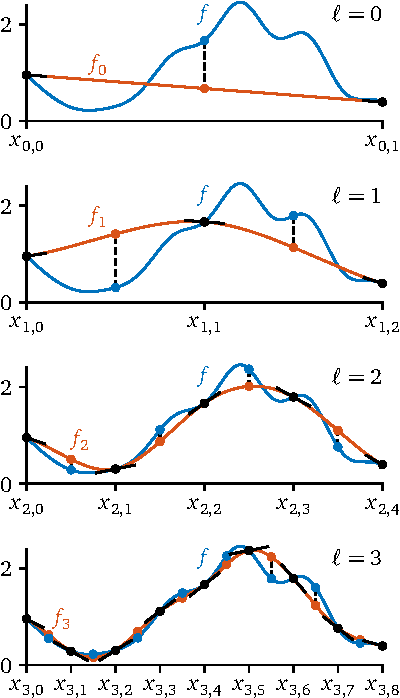
\includegraphics{hermiteHierarchization_1}%
  \caption[%
    Hermite hierarchization%
  ]{%
    Hermite hierarchization on a regular grid in one dimension
    with cubic weakly fundamental splines $\bspl[\wfs]{l,i}{p}$ ($p = 3$).
    The interpolants $\fgintp{l}$ \emph{\textcolor{C1}{(red)}}
    of the objective function \emph{\textcolor{C0}{(blue)}}
    are computed level by level.
    For each level $l$,
    \vspace{-0.1em}%
    the values $\fgintp{l}(\gp{l,i})$ and the derivatives
    $\deriv{x}{\fgintp{l}}(\gp{l,i})$ of the
    current interpolant $\fgintp{l}$ at the
    grid points $\gp{l,i}$ ($i = 0, \dotsc, 2^l$) are saved
    \emph{(black dots and bars).}
    The values and derivatives are used for the Hermite interpolation
    of the residual $\objfun - \fgintp{l}$.
    The interpolated residual is then added to the current interpolant
    such that the sum vanishes in the grid points of the next level $l + 1$
    \emph{%
      (black dashed lines between \textcolor{C1}{red} and
      \textcolor{C0}{blue} dots).%
    }
    Due to the weakly fundamental property, the previously
    interpolated values of $\objfun$ remain unchanged.%
  }%
  \label{fig:hermiteHierarchization}%
\end{SCfigure}

For hierarchical weakly fundamental splines,
the complexity of the $l$-th iteration of \cref{alg:hermiteHierarchization}
is linear in the number of grid points of level $l$, i.e., $\landauO{2^l}$.
The reason for this is the bandedness (with bandwidth $\landauO{p}$) of the
system of linear equations corresponding to the interpolation problem of
\cref{line:algHermiteHierarchization6,line:algHermiteHierarchization7},
which means that the interpolation problem can be solved in
linear time and memory.
In total, the complexity of \cref{alg:hermiteHierarchization} is
given by $\landauO{\sum_{l=0}^n 2^l} = \landauO{2^n}$, i.e.,
the time and memory required by \cref{alg:hermiteHierarchization}
is only linear in the number of grid points.

\pagebreak

\paragraph{Correctness}

We prove the correctness of Hermite hierarchization
with the following invariant.

\begin{restatable}[invariant of Hermite hierarchization]{%
  proposition%
}{%
  propInvariantHermiteHierarchization%
}
  \label{prop:invariantHermiteHierarchization}
  In \cref{alg:hermiteHierarchization}, it holds
  for $l = 0, \dotsc, n$ and $i = 0, \dotsc, 2^l$
  \begin{equation}
    \label{eq:propInvariantHermiteHierarchization}
    \deriv[q]{x}{\fgintp{l}}(\gp{l,i})
    = \sum_{l'=0}^l \sum_{i' \in \hiset{l'}}
    \linout{l',i'} \deriv[q]{x}{\bspl[\wfs]{l',i'}{p}}(\gp{l,i}),\quad
    q = 0, \dotsc, \frac{p-1}{2}.
    \hspace*{-6mm}
  \end{equation}
\end{restatable}

\begin{proof}
  See \cref{sec:a135proofHermiteHierarchization}.
\end{proof}

\begin{restatable}[correctness of Hermite hierarchization]{%
  shortcorollary%
}{%
  corAlgHermiteHierarchizationCorrectness%
}
  \label{cor:algHermiteHierarchizationCorrectness}
  \Cref{alg:hermiteHierarchization} is correct.
\end{restatable}

\begin{proof}
  See \cref{sec:a135proofHermiteHierarchization}.
\end{proof}



\subsection{Hierarchical Weakly Fundamental Not-A-Knot Splines}
\label{sec:456wfsNotAKnot}

Finally, as for fundamental splines,
it is possible to combine the weakly fundamental basis
with the not-a-knot idea from \cref{sec:32notAKnot} to construct
hierarchical weakly fundamental not-a-knot spline functions
$\bspl[\wfs,\nak]{l',i'}{p}$.
The approach is similar to the fundamental not-a-knot splines
in \cref{sec:445fundamentalNotAKnotSplines}
(see \cref{eq:fundamentalNotAKnotSplines}):
Instead of combining uniform B-splines as in
\eqref{eq:weaklyFundamentalSplineParent},
we combine not-a-knot B-splines such that the
weakly fundamental property is satisfied.

However, the exact construction is somewhat complicated,
as one has to carefully consider which conditions to enforce
with which basis functions.
There are some special cases, if the index of the basis function
$\bspl[\wfs,\nak]{l',i'}{p}$ is near the boundary
(near $i' = 0$ or near $i' = 2^{l'}$).
Nevertheless, there are only finitely many special cases;
for higher levels $l'$, one can just scale the basis functions
of coarser levels.
In the scope of this thesis,
it suffices to show the resulting basis functions for
the cubic case ($p = 3$) in
\cref{fig:hierarchicalWeaklyFundamentalNotAKnotSpline},
instead of rigorously stating the technical formulas.

\begin{SCfigure}
  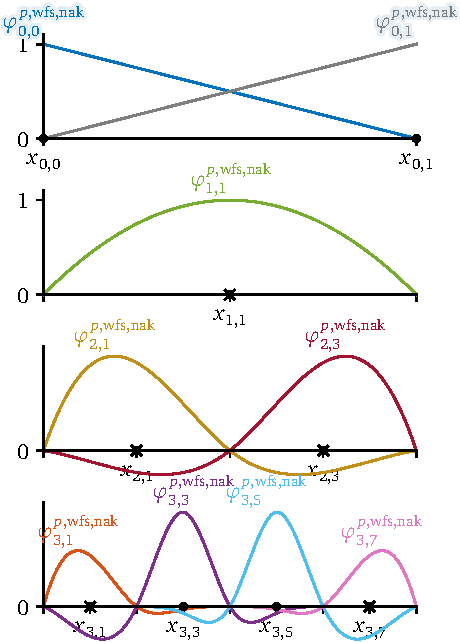
\includegraphics{hierarchicalBasis_18}%
  \caption[%
    Hierarchical weakly fundamental not-a-knot splines%
  ]{%
    Hierarchical cubic weakly fundamental not-a-knot splines
    $\bspl[\wfs,\nak]{l',i'}{p}$
    ($l' \le l$, $i' \in \hiset{l'}$, $p = 3$),
    grid points $\gp{l',i'}$ \emph{(dots),} and
    removed knots \emph{(crosses)} up to level $l = 3$.%
  }%
  \label{fig:hierarchicalWeaklyFundamentalNotAKnotSpline}%
\end{SCfigure}


\cleardoublepage
